\cotefile{144}
\scanpage{122}
On s'intéresse à des objets du type suivant :
\[
\left\{\begin{array}{l}
\text{a) une variété abélienne à isogénie près } A\text{ sur }\overline{\mathbb{Q}},\text{ de dim }g\\[4pt]
\text{b) une structure de }K\text{-module sur }A\\[4pt]
\text{c) pour chaque }\ell,\text{ un isomorphisme de }K\text{-modules}
\end{array}\right.
\]
\diagram{\begin{tikzcd}[column sep=large,row sep=small]
& V_\ell(A) \arrow[d,equal] \\
K\otimes\mathbb{Q}_\ell \arrow[r,leftrightarrow,"\unsure{t_\ell|\iota_\ell}"] & T_\ell(A)\otimes\mathbb{Q}_\ell
\end{tikzcd}}
et on veut déterminer comment $\operatorname{Gal}(\overline{\mathbb{Q}}/\mathbb{Q})$ permute les classes d'isomorphie de tels objets. On n'y arrive pas tout à fait.

Sur $\overline{\mathbb{Q}}$ (ie après extension des scalaires à $\overline{\mathbb{Q}}$), la $\mathbb{Q}$-algèbre $K$ devient un produit de copies de $\overline{\mathbb{Q}}$ :
\[
K\otimes\overline{\mathbb{Q}}\xrightarrow{\sim}\overline{\mathbb{Q}}^{\operatorname{Hom}(K,\overline{\mathbb{Q}})}
\]
Notons $K^*$ le groupe algébrique ``groupe multiplicatif de la $\mathbb{Q}$-algèbre $K$ (c'est $R_{K/\mathbb{Q}}(\mathbb{G}_m)$). $\operatorname{Lie}(A)$ est une représentation de ce groupe -- sur $\overline{\mathbb{Q}}$.
De même pour $\bigwedge^g\operatorname{Lie}(A)$, qui définit, sur $\overline{\mathbb{Q}}$, un caractère
\[
\det\operatorname{Lie}:K^*\longrightarrow\mathbb{G}_m\qquad(\text{défini sur }\overline{\mathbb{Q}}).
\]
Le \uline{corps dual} $K'\subset\overline{\mathbb{Q}}$ est le corps de définition de ce caractère, et on n'arrive à décrire que l'action de $\operatorname{Gal}(\overline{\mathbb{Q}}/K')$.

J'aurais aussi bien pu définir $K'$ comme le plus petit sous-corps de $\overline{\mathbb{Q}}$ tel que le $K$-$\overline{\mathbb{Q}}$-bimodule $\operatorname{Lie} A$ provienne, par extension des scalaires, d'un $K$-$K'$-bimodule $L_0$ (unique à isomorphisme non unique près) : $\operatorname{Lie} A\sim L_0\otimes_{K'}\overline{\mathbb{Q}}$

Ce bimodule détermine un morphisme de groupes algébriques $/\mathbb{Q}$ :
\[
\delta:K'{}^*\longrightarrow K^*:\quad k'\longmapsto\det_K(\text{multiplication par }k'),
\]
qui induit à son tour
\[
\delta:\text{ classes d'idèles de }K'{}^*\longrightarrow\text{ classes d'idèles de }K
\]
\margin{122}


\scanpage{123}
On vérifie que $K'$ est encore quadratique totalement imaginaire sur un corps totalement réel $F'$, et que $\delta$ tue le sous-groupe algébrique $\operatorname{Ker}(F'{}^*\xrightarrow{N}\mathbb{G}_m)$ de $F'{}^*\subset K'{}^*$. Grâce à cela, si $\bar u\in\operatorname{Gal}(\overline{\mathbb{Q}}/K')^{ab}$ correspond à un idèle $\tilde u$ de $K'$ par le corps de classe, la composante finie de $\delta(\tilde u)$, $\in\prod_{v\nmid\infty}K_v^*$, ne dépend que de $u$, si prise modulo $K^*$.

\begin{tabular}{|p{0.92\linewidth}}
\textcircled{Th} Soit $(A,m,\alpha)$ du type dit. Pour $u\in\operatorname{Gal}(\overline{\mathbb{Q}}/K')$, la classe d'isomorphie de $u(A,m,\alpha)$ ne dépend que de l'image \deleted{de} $\bar u$ de $u$ dans $\operatorname{Gal}(\overline{\mathbb{Q}}/K')^{ab}$. C'est celle de $(A,m,\delta(\tilde u)^{-1}\circ\alpha)$
\end{tabular}

Exemple : $K$ quadratique imaginaire - On regarde des courbes elliptiques $A$ à multiplication complexe par l'anneau des entiers $O$ de $K$. On fixe un plongement $K\longrightarrow\overline{\mathbb{Q}}$, et on veut qu'il donne l'action sur Lie.

On a
\[
\begin{gathered}
\text{courbe ell. à mult. par }O\quad\longleftrightarrow\\[4pt]
\begin{gathered}
\text{courbe ell. à isogénie près, à mult. par }K,\text{ plus pour chaque }\ell\\
\text{un réseau }T_\ell\text{ dans }V_\ell(A),\text{ coïncidant pour presque tout }\ell\text{ avec le}\\
\text{réseau }\unsure{\text{standard}|\text{standart}}\text{ (qui n'a un sens que pour presque tout }\ell),\text{ ce réseau étant}\\
O\otimes\mathbb{Z}_\ell\text{-stable}
\end{gathered}\\
\longleftrightarrow\\
\begin{gathered}
\text{courbe ell à isogénie près, à multiplication par }K,\text{ plus pour chaque }\ell\\
\text{un isomorphisme }\alpha_\ell:V_\ell(A)\xrightarrow{\sim}K\otimes\mathbb{Q}_\ell,\text{ donné modulo }(O\otimes\mathbb{Z}_\ell)^*,\\
\text{et donnant un isomorphisme }V_{\unsure{\mathbb{A}^f|\mathbb{A}^+}}(A)\xrightarrow{\sim}\text{adèles finis de }K\\
\text{(un objet de type a) b) c), donné modulo }\widehat O^*\text{)}
\end{gathered}
\end{gathered}
\]
\margin{123}


\scanpage{124}
Le théorème se spécialise pour dire que $\operatorname{Gal}(\overline{\mathbb{Q}}/K)$ permute ces classes \inserted{d'iso de} courbes elliptiques à mult. complexe, l'action se factorisant par $\operatorname{Gal}(\text{corps de classes de Hilbert}/K)\sim\text{groupe des classes d'idéaux}$.

L'action, par $\sigma\longleftrightarrow\text{classe d'idéal }(\sigma)$, est
\[
\sigma(E)\sim E\otimes_O(\sigma)
\]
(j'ai la flemme de préciser les conventions pour savoir si c'est $(\sigma)$ ou $(\sigma)^{-1}$)

\begin{center}
Bien à toi

\unsure{Pierre}
\end{center}
\margin{124}


\scanpage{126}
\diagram{\begin{tikzcd}[row sep=large,column sep=large]
\mathcal M_0^! \arrow[r,dash,"2"] \arrow[d,dash,"4"'] & \underline{\mathcal M}^! \arrow[r,dash,"6"] \arrow[d,dash,"4"'] & \mathcal M \arrow[d,dash,"4"]\\
\underline{\mathcal M}_0^{!0} \arrow[r,dash,"2"] \arrow[d,dash] & \underline{\mathcal M}^{!0} \arrow[r,dash,"\unsure{6}"] \arrow[d,dash] & \underline{\mathcal M}^{0}\\
1 \arrow[r,dash,"2"] & \mu &
\end{tikzcd}}

\diagram{\begin{tikzcd}[column sep=small,row sep=small]
\mathcal M_0^{!0} \arrow[r,phantom,"\simeq"] & \mathcal M(0)^0 & \cdot & \Pi_0\\
& \mathcal M(0) \arrow[u,phantom,"\cap\,4" description] & \cdot & \unsure{\mathcal G|\mathfrak S}^{+} \arrow[u,phantom,"\cap\,12" description]
\end{tikzcd}}
\[
\mathcal M_0^{\prime\prime\prime!}
\]

\[
D_\rho,D_\sigma,
\]

\diagram{\begin{tikzcd}[row sep=small,column sep=small]
& {} \arrow[dl,dash,gray] \arrow[dr,dash,gray] & & {} \arrow[dr,dash,gray] \arrow[rr,dash,gray] \arrow[dd,dash,gray] & & {} \arrow[dr,dash,gray] \arrow[dd,dash,gray] & \\
{}& & \mathcal M_0^! \arrow[rr,dash,gray] & & \mathcal M^! \arrow[rr,dash,gray] \arrow[dl,dash,gray] & & \mathcal M \arrow[dl,dash,gray]\\
{} & \mathcal M_0^{!0} \arrow[ur,dash] \arrow[rr,dash,gray] \arrow[dr,dash,gray] & & \mathcal M^{!0} \arrow[rr,dash,gray] \arrow[dr,dash,gray] & & {} \arrow[dr,dash,gray] & \\
& & {} \arrow[rr,dash,gray] \arrow[uu,dash,gray] & & {} \arrow[rr,dash,gray] & & {}
\end{tikzcd}}

\diagram{\begin{tikzcd}[row sep=small,column sep=small]
& & & & & & & & & \underline{\mathcal M} \arrow[ddll,dash,"2"'] \arrow[dddr,dash,"2"] \arrow[dddddd,dashed,dash] & \\
& & & & & \underline{\mathcal M}^{!} \arrow[urrrr,dash,"6"] \arrow[ddll,dash,"2"'] \arrow[dddr,dash,"2"] & & & & & \\
& \mathcal M_0^{!} \arrow[urrrr,dash,"2"] \arrow[ddl,dash] \arrow[dddr,dash] & & & & & & \underline{\mathcal M}' \arrow[ddddrr,dash,"2"] & & \mathcal M''' & \\
& & & \underline{\mathcal M}^{\prime!} \arrow[urrrr,dash,"6"] \arrow[ddddrr,dash,"2"'] & & \mathcal M^{\prime\prime\prime!} \arrow[uu,dashed] & & & & & \underline{\mathcal M}'' \\
\mathcal M_0^{\prime!} \arrow[urrr,dash,"2"] \arrow[ddddr,dash,"2"'] & \mathcal M_0^{\prime\prime\prime!} \arrow[uu,dashed,dash] & & & & & \underline{\mathcal M}^{\prime\prime!} \arrow[urrrr,dash,"\unsure{6|6!}"] & & & & \\
& & \underline{\mathcal M}_0^{\prime\prime!} \arrow[urrrr,dash,"2"] & & & & & & & & \\
& & & & & & & & & \underline{\mathcal M}^{0} \arrow[uuur,dash,"2"] & \\
& & & & & \underline{\mathcal M}^{!0} \arrow[urrrr,dash,"6"] \arrow[uuur,dash,"2"] \arrow[uuuu,dashed] & & & & & \\
& \underline{\mathcal M}_0^{!0} \arrow[urrrr,dash,"2"] \arrow[uuur,dash] \arrow[uuuu,dashed] \arrow[dd,dash] & & & & \mu \arrow[u,dash] & & & & & \\
& & & & & & & & & & \\
& 1 \arrow[uurrrr,dash] & & & & & & & & &
\end{tikzcd}}

\diagram{\begin{tikzcd}[row sep=large,column sep=large]
& \mu\times1 \arrow[d]\\
\mathcal M \arrow[r,"{(\varphi,\varepsilon_3)}"] & \unsure{\mathcal G|\mathfrak S}/\Pi_0\times\mu \arrow[dd]\\
\deleted{\mathcal M} \arrow[r,draw=none,"\deleted{\longrightarrow}" description] & \deleted{\unsure{\mathcal G_3|\mathfrak S_3}\mathbin{\unsure{\rtimes|\times}}\mu\times\mu}\\
& \unsure{\mathcal G_3|\mathfrak S_3}\times\mu\times\mu
\end{tikzcd}}

\diagram{\begin{tikzcd}[row sep=small,column sep=small]
& & & & \unsure{\mathcal G_3|\mathfrak S_3}\times\mu & & {} \arrow[ddr,dash,gray] & \\
& & {} \arrow[ddr,dash,gray] \arrow[urrrr,dash,gray] & & & & & \\
{} \arrow[urr,dash,gray] \arrow[dr,dash,gray] \arrow[rrrr,dash,gray] & & & & {} \arrow[rrr,dash,gray] \arrow[dr,dash,gray] & {}& & {} \\
& {} \arrow[rr,dash,gray] & & {} \arrow[ur,dash,gray] \arrow[urr,dash,gray] & & {} \arrow[urr,dash,gray] & & \\
& & & & & \unsure{\mathbb F_2-\psi(\mathbb F_2)|\mathbb F_2-\mu(\mathbb F_2)} & &
\end{tikzcd}}

\diagram{\begin{tikzcd}[row sep=large,column sep=large]
& \underline{\mathcal M}/\underline{\mathcal M}^{!0}\simeq\unsure{\mathcal G_3|\mathfrak S_3}\mathbin{\unsure{\rtimes|\times}}\mu\times\mu \arrow[r] & 1\\
1 \arrow[r] & \mu \arrow[r] & \underline{\mathcal M}/\underline{\mathcal M}_0^{!0} \arrow[ul]
\end{tikzcd}}

\diagram{\begin{tikzcd}[row sep=large,column sep=large]
1 \arrow[r] & \operatorname{Sl}(2,\mathbb Z/4\mathbb Z) \arrow[r] \arrow[d,"8"] & \operatorname{Gl}(2,\mathbb Z/4\mathbb Z) \arrow[r] & (\mathbb Z/4\mathbb Z)^*\\
& \underset{6}{\operatorname{Sl}(\unsure{2|?},\mathbb Z/2\mathbb Z)} & 6\cdot16 &
\end{tikzcd}}
\[
48\quad\deleted{\unsure{48}}\qquad\deleted{\unsure{2}}
\]
\[
\mathcal M_0^{\prime\prime!}\cap N_\rho^*=Z_{\rho\,0}^{\prime\prime\deleted{\unsure{*}}!}
\]
\margin{126}


\scanpage{127}
\begin{center}
ACADEMIE DE MONTPELLIER\\
\rule{2cm}{0.4pt}

UNIVERSITÉ\\
DES SCIENCES \& TECHNIQUES\\
DU LANGUEDOC\\
\rule{2cm}{0.4pt}

34060 MONTPELLIER CEDEX\\
\rule{2cm}{0.4pt}
\end{center}

MR LE PROFESSEUR GROTHENDIECK ALEX.

MATHEMATIQUES\hfill 5

\margin{127}


\scanpage{129}
\[
\unsure{\mathcal G_{1,1}|\mathfrak S_{1,1}}\simeq\mathcal T_{1,2}^{!}
\qquad
\begin{pmatrix}-1&1\\0&1\end{pmatrix}
\qquad
\rho\left(\unsure{\tfrac12|1},\tfrac12\right)=\left(\tfrac12,-\tfrac12\right)
\]

\figure{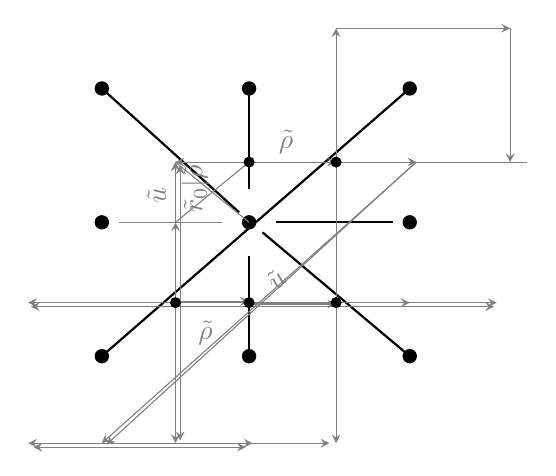
\begin{tikzpicture}[x=0.85cm,y=0.85cm,>=stealth]
\foreach \x in {1.1,3.3,5.7}{\foreach \y in {1.3,3.3,5.3}{\fill (\x,\y) circle (2.6pt);}}
\draw[thick] (1.1,1.3)--(5.7,5.3);
\draw[thick] (1.1,5.3)--(3.15,3.45) (3.5,3.15)--(5.7,1.3);
\draw[thick] (3.3,1.3)--(3.3,2.8) (3.3,3.8)--(3.3,5.3);
\draw[gray] (1.35,3.3)--(2.9,3.3);
\draw[thick] (3.7,3.3)--(5.45,3.3);
\draw[gray,<->] (0,2.1)--(7,2.1);
\draw[gray,<->] (0.04,2.04)--(6.96,2.04);
\draw[gray,->] (2.2,2.12)--(3.3,2.12);
\draw[gray,->] (3.3,2.08)--(4.6,2.08);
\draw[gray,->] (4.6,2.1)--(5.7,2.1);
\draw[gray,<->] (2.2,0)--(2.2,4.2);
\draw[gray,<->] (2.27,0.04)--(2.27,4.15);
\draw[gray,->] (2.2,2.1)--(2.2,3.3);
\draw[gray,->] (2.2,3.3)--(2.2,4.2);
\draw[gray,->] (4.6,4.2)--(4.6,0);
\draw[gray,<->] (0,0)--(4.5,0);
\draw[gray,<->] (0.08,-0.06)--(3.25,-0.06);
\draw[gray,->] (2.2,0)--(3.35,0);
\draw[gray,<->] (2.2,4.2)--(4.6,4.2);
\draw[gray,->] (4.6,4.2)--(5.8,4.2);
\draw[gray] (5.8,4.2)--(7.45,4.2);
\draw[gray,->] (4.6,4.2)--(4.6,6.2);
\draw[gray,->] (4.6,6.2)--(7.2,6.2);
\draw[gray,->] (7.2,6.2)--(7.2,4.2);
\draw[gray,->] (5.8,4.2)--(1.1,0);
\draw[gray,->] (5.75,4.16)--(1.17,-0.02);
\draw[gray] (2.2,4.2)--(3.3,3.3) (2.2,3.3)--(3.3,4.2);
\foreach \p in {(2.2,2.1),(3.3,2.1),(4.6,2.1),(4.6,4.2),(3.3,4.2)}{\fill \p circle (2pt);}
\node[gray,rotate=90] at (1.92,3.7) {$\unsure{\tilde u}$};
\node[gray,rotate=90] at (2.5,3.8) {$\unsure{\tilde r_0|\tilde\rho}$};
\node[gray] at (3.85,4.5) {$\unsure{\tilde\rho}$};
\node[gray] at (2.65,1.65) {$\unsure{\tilde\rho}$};
\node[gray,rotate=45] at (3.7,2.45) {$\unsure{\tilde u}$};
\end{tikzpicture}}

\[
r_0\unsure{u}r_0
\qquad
(ur_1)^{-1}=r_1u^{-1}
\]
\[
(ur_\infty)^{-1}=r_\infty u^{-1}
\]
\[
\tilde v^{-1}\tilde u\tilde v\tilde u^{-1}
\qquad
(ur_\infty)^{-1}
\]
\diagram{\begin{tikzcd}[column sep=large]
\tilde u\tilde v & (vr_\infty)^{-1}\unsure{\circ j|\circ c_j}=r_\infty v^{-1} \arrow[l]
\end{tikzcd}}
\[
\tilde\rho\qquad r_1v^{-1}
\]

\[
(u,\ell)(\unsure{u'},\ell')=(uu',u\ell')\ell
\]
\diagram{\begin{tikzcd}[column sep=large,row sep=large]
& u(a) \arrow[dr,dash] & \\
a \arrow[ur,"\unsure{\ell}"] \arrow[dr,dash,"\ell'"'] \arrow[rr] \arrow[rr,bend left=10,"\deleted{\unsure{u(\ell')}}"] \arrow[rr,bend right=10,"\deleted{\unsure{u'(\ell)}}"'] & & uu'(a)\\
& u'(a) \arrow[ur,dash,"\deleted{\unsure{u(\ell')}}"'] &
\end{tikzcd}}

\[
\begin{aligned}
\ell &: a\longrightarrow ua\\
\ell' &: a\mathbin{-\!\!-}u'a
\end{aligned}
\qquad
\begin{aligned}
u'(\ell)&:u'a\mathbin{-\!\!-}u'ua\\
\uline{u(\ell')}&:\uline{ua\mathbin{-\!\!-}uu'a}
\end{aligned}
\]
\diagram{\begin{tikzcd}
a \arrow[r,dash,"\ell"] & ua \arrow[r,dash] & uu'a
\end{tikzcd}}
\margin{129}


\scanpage{130}
\[
\tilde r_1^2(\unsure{\tilde u})=\tilde u
\]
\[
\tilde r_1^2(\unsure{\tilde v|\tilde w})=\tilde u^{-1}[\unsure{\tilde u|\tilde w}\tilde v]=\tilde v
\]
\[
\tilde r_1\ell
\]
\[
\deleted{\tilde u^{-1}}\deleted{\tilde u}\tilde v\tilde u\tilde v^{-1}\tilde u^{-1}\;-
\]

\[
(\gamma,\ell)(\gamma',\ell')(\gamma'',\ell'')
\]
\diagram{\begin{tikzcd}[column sep=large,row sep=large]
a \arrow[r,"\ell''"] & \gamma''{}^{-1}(a) \arrow[r,"\gamma''{}^{-1}(\ell')"] & (\gamma'\gamma'')^{-1}(a) \arrow[d,"(\gamma'\gamma'')^{-1}(\ell)"']\\
& & (\gamma\gamma'\gamma'')^{-1}(a)
\end{tikzcd}}

UNIVERSITE DES SCIENCES\\
ET TECHNIQUES DU LANGUEDOC\\
M A T H E M A T I Q U E S\hfill 30.10.80

\begin{center}
SEMINAIRE GEOMETRIE ALGEBRIQUE
\end{center}

Tous les mercredis à 14 h 30, Salle 331.

\begin{tabular}{lll}
Exposés prévus : & 12 novembre, & Schémas formels (C. CONTOU-CARRERE)\\
& 19 novembre, & Schémas formels (suite)\\
& 26 novembre, & Correspondances sur les courbes (D. ALIBERT)\\
& 3 décembre, & Correspondances sur les courbes (suite).
\end{tabular}

\begin{flushright}
D. ALIBERT\qquad C. CONTOU-CARRERE
\end{flushright}

(la première séance aura lieu le 12 novembre).
\margin{130}


\scanpage{131}
\[
\tilde u,\tilde v\qquad
[\tilde u,\tilde v]=\deleted{\unsure{\omega_0}}\ell_0'{}^{-1}
\]
\[
\tilde\rho,\tilde\sigma,\tilde\omega_0\qquad
\tilde\rho^3=\tilde\omega_0^{\deleted{\unsure{-1}}}
\qquad
\tilde\sigma^2=\tilde\omega_0^{-1}
\qquad
\tilde\omega_0^2=\ell'_0
\]
\[
\tilde r_0,\quad\deleted{\unsure{\tilde r_0^2=1}}
\]

\diagram{\begin{tikzcd}[row sep=small,column sep=small]
\unsure{\mathcal G_{1,1}|\mathfrak G_{1,1}} \arrow[r,phantom,"\simeq"] & \mathcal T_{1,2}^{!}\\
\mathrm S\mathcal T_{1,1}\simeq\operatorname{Gl}(2,\mathbb Z)^\sim \arrow[u,phantom,"\cup" description]\\
\operatorname{Norm}_{\unsure{\mathcal G_{1,1}|\mathfrak G_{1,1}}}(L'_0) \arrow[u,equal] & (L'_0\text{ engendré par }\ell'_0)
\end{tikzcd}}

\[
\left.\begin{aligned}
\tilde r_0(\tilde\rho)&=\tilde\rho^{-1}\\
\tilde r_0(\tilde\sigma)&=\tilde\sigma^{-1}
\end{aligned}\right|\Longrightarrow r_0(\tilde\omega_0)=\tilde\omega_0^{-1}
\]
\[
\uline{\text{def}}\left\{\begin{aligned}
\tilde r_1&=\tilde r_0\tilde\rho\qquad\text{i.e. }\tilde\rho=\tilde r_0\tilde r_1\\
\tilde r_\infty&=\tilde\sigma\tilde r_0\qquad\text{i.e. }\tilde\sigma=\tilde r_\infty\tilde r_0
\end{aligned}\right.
\]
\[
\text{NB}\quad\tilde r_1\tilde r_\infty=(\tilde\sigma\tilde\rho)^{-1}=\tilde\tau_0^{-1}
\quad\text{où }\tilde\tau_0\overset{\mathrm{def}}=\tilde\sigma\tilde\rho
\]

\diagram{\begin{tikzcd}[row sep=large]
\boxed{\tilde r_0^2=\tilde r_1^2=\tilde r_\infty^2=1,\quad(\tilde r_0\tilde r_1)^3(\tilde r_\infty\tilde r_0)^2=1}\\
\begin{aligned}
\tilde\rho(\tilde u)&=\deleted{\unsure{\tilde\rho\tilde u\tilde\rho^{-1}}}=(\tilde r_0\tilde r_1)(\tilde u)=\tilde v^{-1}\\
\tilde\rho(\tilde v)&=\deleted{\unsure{\tilde\rho\tilde v\tilde\rho^{-1}}}=(\tilde r_0\tilde r_1)(\tilde v)=\tilde v\tilde u\\
\tilde\sigma(\tilde u)&=\deleted{\unsure{\tilde\sigma\tilde u\tilde\sigma^{-1}}}=(\tilde r_\infty\tilde r_0)(\tilde u)=\tilde u(\tilde v)=\tilde u\tilde v\tilde u^{-1}\\
\tilde\sigma(\tilde v)&=\deleted{\unsure{\tilde\sigma\tilde v\tilde\sigma^{-1}}}=(\tilde r_\infty\tilde r_0)(\tilde v)=\tilde u^{-1}
\end{aligned}\\
\left\{\begin{aligned}
\tilde r_0(\tilde u)&=\tilde r_0\tilde u\tilde r_0=\tilde v\\
\tilde r_0(\tilde v)&=\tilde r_0\tilde v\tilde r_0=\tilde u
\end{aligned}\right.\quad\Big|\Longrightarrow\tilde r_0(\ell'_0)=\ell'_0{}^{-1}
\arrow[uu,bend left=65,start anchor=west,end anchor=west]
\end{tikzcd}}
\[
\left\{\begin{aligned}
\tilde r_\infty(\tilde u)&=\tilde r_\infty\tilde u\tilde r_\infty=\tilde u^{-1}\\
\tilde r_\infty(\tilde v)&=\tilde r_\infty\tilde v\tilde r_\infty
=\deleted{\unsure{\tilde u\tilde v\tilde u^{-1}\tilde v^{-1}\tilde v}}\tilde v^{\unsure{*}}[\tilde v^{-1},\tilde u]
=\deleted{\unsure{\tilde v\tilde v^{-1}}}\tilde u\tilde v\tilde u^{-1}=\tilde u(\tilde v)
\end{aligned}\right.\Big|\Longrightarrow\unsure{\tilde r_1|\tilde r_\infty}(\ell'_0)=\unsure{\ell'_0|\ell'_0{}^{-1}}
\]
\[
\left\{\begin{aligned}
\tilde r_1(\tilde u)&=\tilde r_1\tilde u\tilde r_1=\tilde u^{-1}\\
\tilde r_1(\tilde v)&=\tilde r_1\tilde v\tilde r_1=\tilde u\tilde v
\end{aligned}\right.\Big|\Longrightarrow\tilde r_1(\ell'_0)=\ell'_0{}^{-1}
\]

\[
\left\{\tilde r_0,\tilde r_1,\tilde r_\infty,\tilde u,\tilde v\;\left|\;
\begin{gathered}
\tilde r_0^2=\tilde r_1^2=\tilde r_\infty^2=
\deleted{\unsure{1,(\tilde r_0\tilde r_1)^3(\tilde r_\infty\tilde r_0)^2=1}}
\inserted{=(\tilde r_0\tilde r_1)^3(\tilde r_\infty\tilde r_0)^2=1}\\
(\tilde r_0\tilde r_1)^6\deleted{\unsure{=}}\;(=(\tilde r_\infty\tilde r_0)^4)=[\tilde u,\tilde v]\\
\text{(C)}\left\{\begin{aligned}
\tilde r_0(\tilde u)&=\tilde v,\quad\tilde r_0(\tilde v)=\tilde u\\
\tilde r_\infty(\tilde u)&=\tilde u^{-1};\quad\tilde r_\infty(\tilde v)=\tilde u(\tilde v)\;(=\tilde u\tilde v\tilde u^{-1})\\
r_1(\tilde u)&=\tilde u^{-1};\quad r_1(\tilde v)=\tilde u\tilde v
\end{aligned}\right.
\end{gathered}\right.\right\}
\]
\[
=\left\{\tilde r_0,\tilde r_1,\tilde r_\infty,\tilde\omega_0,\tilde u,\tilde v\;\left|\;
\begin{gathered}
r_0^2=r_1^2=r_\infty^2=1,\quad(\tilde r_0\tilde r_1)^3=(\tilde r_\infty\tilde r_0)^2=\tilde\omega_0\\
\tilde\omega_0^2=[\tilde u,\tilde v]\\
\text{relations en conjugaison (C)}
\end{gathered}\right.\right\}
\]
\margin{131}


\scanpage{132}
UNIVERSITE DES SCIENCES ET TECHNIQUES\\
DU LANGUEDOC

Institut de Mathématiques

Place Eugène Bataillon\\
34060 MONTPELLIER CEDEX

Dans le cadre des conférences d'intérêt général, Monsieur JAMBON parlera le Vendredi 31 Octobre à 14h30, sallede cours n$^{\mathrm{o}}$ 4 sur le sujet suivant :

\begin{center}
LE FINI ET L'INFINI EN LIAISON AVEC

L'AXIOME DU TIERS EXCLU
\end{center}

Vous êtes invité à cette conférence et au thé des mathématiciens qui suivra à 16 h dans la Salle de Réunion du Bâtiment de Mathématiques.

\begin{flushright}
M. LEFRANC

Directeur de l'U.F.R. 5
\end{flushright}
\margin{132}


\scanpage{134}
\diagram{\begin{tikzcd}[row sep=large,column sep=large]
1 & 1 & \deleted{\unsure{\mathbb Z/2\mathbb Z}}\\
\mathcal G_{0,3} \arrow[u] \arrow[r] & \mathcal T_{0,3}=\mathcal G_{0,3}/\mathcal G_{0,3}^{+!}\simeq\mathcal G_3\times\mu_\tau \arrow[u]\\
\unsure{\mathcal G_*|\mathcal G^*} \arrow[u] \arrow[r] & \widetilde{\mathcal T}_{0,3}=\unsure{\mathcal G}/\underbrace{(\unsure{\mathcal G_{0,3}^{!+}|\mathcal G_0^{!+}})_0}_{\substack{\text{engendré par }\lambda_0\lambda_1\lambda_\infty\\(\lambda_i=-\ell_i)}} \arrow[u]\\
\mu \arrow[u] \arrow[r,equal] & \mu \arrow[u]\\
1 \arrow[u] & 1 \arrow[u]
\end{tikzcd}}
\[
\mathcal G=\left\{\rho,\sigma,\tau'\;\left|\;\begin{array}{l}
\rho^6=\sigma^4=\tau'{}^2=1,\ \rho^3=\sigma^2,\\
\tau'(\rho)=\rho^{-1};\quad\tau'(\sigma)=\sigma^{-1}
\end{array}\right.\right\}
\]
\[
=\left\{\rho,\sigma,\tau\;\left|\;\begin{array}{l}
\rho^6=\sigma^4=\tau^2=1,\ \rho^3=\sigma^2\\
\tau(\rho)=\sigma(\rho^{-1}),\quad\tau(\sigma)=\sigma^{-1}\deleted{\unsure{(\rho)}}
\end{array}\right.\right\}
\]
\[
\uline{\text{NB}}\quad\tau=\deleted{\unsure{\rho}}\sigma\tau'=\tau'\sigma^{-1}
\]

\textcircled{I}\quad Position relative de $L_\rho$ et $L_\sigma$

\diagram{\begin{tikzcd}[row sep=large,column sep=large]
& & D_\sigma \arrow[drr,hook] & \unsure{SD_\sigma} \arrow[dd,dash,gray] & \\
\underline\mu_{\tau'} \arrow[r,hook,"2"] & D_2 \arrow[ur,hook,"2"] \arrow[rr,hook] \arrow[ddrr,hook,"3"] & & \unsure{\Pi_{\tau'}|\Pi'} \arrow[r,hook,"6"] & \mathcal G\\
& & L_\sigma \arrow[uu,hook,"2"] & \unsure{SZ_\sigma} & \\
\{1\} \arrow[uu,hook,"2"] \arrow[r,hook,"2"] & \underline\mu \arrow[uu,hook,"2"] \arrow[ur,hook,"2"] \arrow[rr,hook] \arrow[ddrr,hook,"3"] & & \underline\Pi \arrow[uu,hook,"2"] \arrow[r,hook,"6"] & \underline{\mathcal G}^{+} \arrow[uu,hook,"2"]\\
& & & D_\rho \arrow[uuur,hook] \arrow[ur,hook] & \\
& & & L_\rho \arrow[u,hook,"2"] \arrow[uur,hook] &
\end{tikzcd}}

\diagram{\begin{tikzcd}[column sep=large,row sep=large]
& D_\sigma \arrow[dr,hook,"3"] & \\
D_2 \arrow[ur,hook,"2"] \arrow[ddr,hook,"3"] & & \mathcal G/\Pi_0\\
& L_\sigma \arrow[uu,hook,"2"] & \\
\mu \arrow[uu,hook,"2"] \arrow[ur,hook,"2"] \arrow[ddr,hook,"3"] & D_\rho \arrow[uur,hook,"2"] \arrow[dr,hook,"3"] & \\
& & \mathcal G^+/\Pi_0 \arrow[uuu,hook,"2"]\\
\{1\} \arrow[uu,hook,"2"] & L_\rho \arrow[uu,hook,"2"] \arrow[ur,hook,"2"] &
\end{tikzcd}}

\diagram{\begin{tikzcd}[row sep=small]
\unsure{\mathcal M^!} \arrow[r,dash,gray] \arrow[dr,dash,gray] & \unsure{\mathcal M_\rho} \arrow[dr,dash,gray] & \\
& \unsure{\mu} & {}
\end{tikzcd}}

\[
\underset{\text{ordre }24}{\mathcal G/\Pi_0}=\left\{\rho,\sigma,\tau\;\left|\;\begin{array}{l}
\rho^6=\sigma^4=\tau^2=1,\ \rho^3=\sigma^2\\
\tau(\sigma)=\sigma^{-1},\quad\tau(\rho)=\rho\\
\sigma(\rho)=\rho^{-1}
\end{array}\right.\right\}
\]
\[
\underset{\text{ordre }12}{\mathcal G^+/\Pi_0}=\left\{\rho,\sigma\;\left|\;\begin{array}{l}
\rho^6=\sigma^4=1,\ \rho^3=\sigma^2\\
\sigma(\rho)=\rho^{-1}
\end{array}\right.\right\}
\]

\figure{\begin{tikzpicture}\draw (0,1.7)--(5.8,1.7) .. controls (7,1.7) and (6.8,0.2) .. (7.5,0.1)--(13,0);\end{tikzpicture}}
\textcircled{II}
\diagram{\begin{tikzcd}[row sep=large,column sep=large]
\mu\times\mu_{\tau'}=D_2 \arrow[rr,hook,"2"] & & \underset{\mu\times\Pi'_0=}{\unsure{\mathcal G^!=\Pi'_0|\mathcal G^!=\Pi_{\tau'}}} \arrow[rr,hook,"6"] & & \mathcal G\\
& \mu_\tau \arrow[ul,hook,"2"] \arrow[rr,hook,"2"] & & \mathcal G_0^!=\Pi' \arrow[ul,hook,"2"] & \\
\underline\mu \arrow[uu,hook,"2"] \arrow[rr,hook,"2"] & & \underset{\mu\times\Pi_0=}{\underline{\mathcal G}^{!+}=\Pi} \arrow[uu,hook,"2"] \arrow[rr,hook,"6"] & & \underline{\mathcal G}^{+} \arrow[uu,hook,"2"]\\
& \{1\} \arrow[uu,hook,"2"] \arrow[ul,hook,"2"] \arrow[rr,hook,"2"] & & \underline{\mathcal G}_0^{!+}=\Pi_0 \arrow[uu,hook,"2"] \arrow[ul,hook,"2"] &
\end{tikzcd}}
\[
\unsure{\mathcal G^{!+}}\qquad
\begin{aligned}\rho&\mathrel{\mapstochar\! -\! -}\rho\\\sigma&\longmapsto-\sigma\end{aligned}
\]
\[
\underline\mu\simeq\mu_\tau\simeq\{\pm1\}
\]
\[
\mu_\tau=\{1,\tau\},\quad\mu_{\tau'}=\{1,\tau'\}
\qquad\mu=\{\pm1\}
\]
\[
\mathcal G=
\]

\diagram{\begin{tikzcd}[row sep=large,column sep=large]
\unsure{\mathcal M_\Pi^![0]} \arrow[r,dash,gray] \arrow[d,dash,gray] \arrow[dr,dash,gray] & \unsure{\mathcal M^!(0)} \arrow[r,gray] \arrow[d,dash,gray] & \unsure{\mathcal M_\Pi^![0]} \arrow[rr,dash,gray] \arrow[d,dash,gray] \arrow[dr,dash,gray] & & \unsure{\mathcal M^!} \arrow[d,dash,gray] \arrow[dr,dash,gray] & \\
{}& \mu_\tau \arrow[r,dash,gray] & D_0^\Pi \arrow[r,dash,gray] \arrow[d,dash,gray] \arrow[dr,dash,gray] & \unsure{\mathcal M_{\mathcal G}^{!}[0]} \arrow[rr,gray,"\Pi'"] \arrow[d,dash,gray] & {}& \mathcal M\\
\unsure{\mathcal M_\Pi^![0]} \arrow[r,dash,gray] \arrow[ddr,dash,gray] & 1 \arrow[r,dash,gray] \arrow[dd,dash,gray] & L_0^\Pi \arrow[r,dash,gray] \arrow[dr,dash,gray,"2"] & \unsure{D_0^{\mathcal G}} \arrow[rr,dash,gray,"\Pi"] \arrow[d,dash,gray] \arrow[drr,dash,gray] & & \unsure{\mathcal G} \arrow[d,dash,gray]\\
& & & \unsure{L_0^{\mathcal G}} \arrow[rr,dash,gray] & & \mathcal G^+\\
& \unsure{L_0^{\mathcal G}} \arrow[rr,dash,gray] & & \unsure{\mathcal G} & &
\end{tikzcd}}

\diagram{\begin{tikzcd}[column sep=large,row sep=large]
\Pi'=\mathcal G^! \arrow[r,hook,gray] \arrow[d,dash,gray] \arrow[dr,dash,gray] & \mathcal G \arrow[d,dash,gray] & \\
\Pi=\mathcal G^{!+} \arrow[r,hook,gray] \arrow[dr,dash,gray] & \underline{\mathcal G}^{+} \arrow[dr,dash,gray] & \\
& \mathcal M^{!+} \arrow[r,dash,gray] & \mathcal M^+
\end{tikzcd}}
\margin{134}


\scanpage{135}
U N I V E R S I T E\\
DES SCIENCES ET TECHNIQUES\\
DU LANGUEDOC\\
\rule{3cm}{0.4pt}
\hfill MONTPELLIER, le 5 Juillet 1979

Service de la Scolarité\\
MR/MB\\
\uline{Diffusion} : Liste A\\
N$^{\mathrm{o}}$3963

\begin{center}
\uline{AVIS DE SOUTENANCE D'UNE THESE DE DOCTORAT DE 3ème CYCLE} :

\uline{SCIENCES DE L'EAU}
\end{center}

\uline{NOM et Prénom du candidat} : Monsieur VELARD Frank

\uline{Titre de la thèse} : Modèles simples de comportement d'une source d'eau chaude.\\
Essai d'application aux sources thermales de la haute vallée de la Têt (Pyrénées-\\
Orientales).

\uline{Date, heure et lieu de soutenance prévus} : Mercredi 11 Juillet 1979 à 16 h.\\
\hspace*{6cm}Salle de cours N$^{\mathrm{o}}$ 10.

\uline{Nom du Directeur de la thèse} : Monsieur C. DROGUE.

\uline{Désignation du laboratoire où la thèse est préparée} : Laboratoire d'Hydrogéologie\\
et centre d'informatique géologique de l'école nationale supérieure des mines de\\
Paris à \unsure{Fontainebleau|Fôntainebleau}.

\uline{Analyse de l'ouvrage}$^{\mathrm{o}}$ :\\
Ce \unsure{travail|trabail} est un essai de représentation du fonc-\\
tionnement d'une source thermale à l'aide \unsure{d'unemodèle|d'un modèle} numérique traitant de l'écou-\\
lement ascendant dans une fente. Ce modèle est ensuite appliqué aux sources thermales\\
de la haute vallée de la Têt (\unsure{Pyénées|Pyrénées} Orientales), compte tenu des caractères géologi-\\
ques, hydrauliques et physico-chimiques de ces sources.

\uline{Durée approximative des recherches ayant abouti à la thèse} : 2 ans.

\begin{tabular}{ll}
\uline{Composition du jury proposé} : & MM. F. PROUST\\
& J. AUROUZE\\
& \unsure{C.|G.} DROGUE\\
& M. COMBARNOUS\\
& E. LEDOUX\\
& G. VASSEUR.
\end{tabular}

\begin{flushright}
Le Secrétaire Général,

\unsure{E. Siau}
\figure{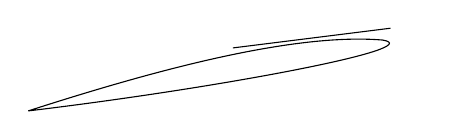
\begin{tikzpicture}[x=1cm,y=1cm]\draw (0,0) .. controls (1.4,.45) and (3.3,1.0) .. (4.5,.9) .. controls (5.1,.8) and (2.5,.3) .. (0,0);\draw (2.6,.8)--(4.6,1.05);\end{tikzpicture}}
\uline{E. SIAU}
\end{flushright}
\margin{135}


\scanpage{136}
\deleted{Position de}\quad +\quad Les relations
\[
\underset{\mathcal G^{+!}}{\underset{\Vert}{\Pi}}\simeq
\underset{\mathcal G_0^{+!}}{\underset{\Vert}{\Pi_0}}\times\{\pm1\},\quad
\Pi'=\{1,\tau\}\cdot\Pi=D_\tau\cdot\Pi_0=\Pi'_0\times\mu
\]
\[
\Pi'_0=\{1,\tau\}\cdot\Pi_0
\]
\textcircled{II}
\diagram{\begin{tikzcd}[row sep=large,column sep=large]
\mu_\tau \arrow[rr,hook,"2"] \arrow[dr,hook,"2"] & & D_\tau=\mu_\tau\times\mu \arrow[dr,hook,"2"] & & & \\
& \mathcal G_0^!=\Pi'_0 \arrow[rr,hook,"2"] & & \Pi'=\Pi'_0\times\mu=\mathcal G^! \arrow[rr,hook,no head,"6"] \arrow[ddrrr,hook] & & \mathcal G \arrow[ddrr,hook] & & \\
\{1\} \arrow[uu,hook,"2"] \arrow[rr,hook,"2"] \arrow[dr,hook,"2"] & & \underline\mu \arrow[uu,hook,"2"] \arrow[dr,hook,"2"] & & & & & & \\
& \mathcal G_0^{+!}=\Pi_0 \arrow[uu,hook,"2"] \arrow[rr,hook,"2"] & & \Pi=\Pi_0\times\mu=\mathcal G^{+!} \arrow[uu,hook,"2"] \arrow[rr,hook,"6"] \arrow[ddrr,hook] & & \mathcal G^+ \arrow[uu,hook,"2"] \arrow[ddrrr,hook] & \mathcal M^! \arrow[r,"6"] & \mathcal M & {}\\
& & & & & & & & \\
& & & & & \mathcal M^{+!} \arrow[uur,hook,"\widehat{\mathbb Z}^{*}\deleted{\unsure{2}}"] \arrow[rrr,hook,"6"] & & {}& \mathcal M^+ \arrow[uul,hook,"\widehat{\mathbb Z}^{*}\deleted{\unsure{2}}"]
\end{tikzcd}}

\diagram{\begin{tikzcd}[row sep=large]
\Pi_0\simeq\{\lambda_0,\lambda_1,\lambda_\infty\mid\lambda_\infty\lambda_1\lambda_0=1\} \arrow[d,hook]\\
\mathcal G
\end{tikzcd}}
\[
\lambda_i\longmapsto-\ell_i
\]

\diagram{\begin{tikzcd}[row sep=large,column sep=large]
& \deleted{\mathcal M^!} \arrow[rr] & & \deleted{\mathcal M}\\
\deleted{\Pi'=\mathcal G^!} \arrow[ur,hook] \arrow[rr,hook] & & \deleted{\mathcal G} \arrow[ur,hook] & \\
& \deleted{\mathcal M^{+!}} \arrow[uu,hook] \arrow[rr] & & \deleted{\mathcal M^+} \arrow[uu,hook]\\
\deleted{\mathcal G^{+!}} \arrow[uu,hook] \arrow[ur,hook] \arrow[rr,hook] & & \deleted{\mathcal G^+} \arrow[uu,hook] \arrow[ur,hook] &
\end{tikzcd}}
\figure{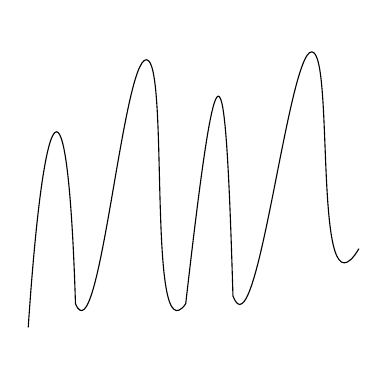
\begin{tikzpicture}\draw (0,0) .. controls (.2,3) and (.5,3.5) .. (.6,.3) .. controls (.9,-.4) and (1.2,3.4) .. (1.5,3.4) .. controls (1.8,3.4) and (1.5,-.4) .. (2,.3) .. controls (2.4,3.8) and (2.5,3.8) .. (2.6,.4) .. controls (2.9,-.4) and (3.3,3.5) .. (3.6,3.5) .. controls (3.9,3.5) and (3.6,0) .. (4.2,1);\end{tikzpicture}}

$\mathcal G/\Pi_0$ ou $\mathcal G^+/\Pi_0$ déduits de $\mathcal G$ \unsure{et|ou} $\mathcal G^+$ en divisant par la relation $\tau'(\rho)=\deleted{\unsure{\rho}}\sigma(\rho)$ ou encore $\tau(\rho)=\rho$ ($\uline{\mathrm{NB}}\ \tau(\rho)=\deleted{\unsure{1}}-(\ell_{\unsure{i|1}}^{-1})\rho$ !)

\rule{\linewidth}{0.4pt}
\uline{III}\quad\deleted{position de $\mathcal M(0)$}

$\mathcal M(0)$ et groupes associés

\diagram{\begin{tikzcd}[column sep=large,row sep=large]
\mathcal M(0) \arrow[r,hook] & \unsure{\mathcal M^\Pi_\Pi[0]|\mathcal M^\Pi[0]} \arrow[rr,hook] \arrow[dr,hook,"6"] & & \mathcal M^! \arrow[dr,hook] & \\
& & \mathcal M^{\mathcal G}[0] \arrow[rr,hook] & & \mathcal M \arrow[dd,dash]\\
\mu_\tau \arrow[uu,hook] \arrow[r,hook] & D_0^\Pi \arrow[uu,hook] \arrow[rr,hook] \arrow[dr,hook,"2"] & & \Pi'=\mathcal G^! \arrow[uu,hook] \arrow[dr,hook] & \\
& & D_0^{\mathcal G} \arrow[uu,hook] \arrow[rr,hook] & & \mathcal G\\
\{1\} \arrow[uu,hook] \arrow[r,hook,"\widehat{\mathbb Z}"] & L_0^\Pi \arrow[uu,hook] \arrow[rr,hook] \arrow[dr,hook,"2"] & & \underline\Pi=\mathcal G^{+!} \arrow[uu,hook] \arrow[dr,hook,"6"] & \\
& & L_0^{\mathcal G} \arrow[uu,hook] \arrow[rr,hook] & & \mathcal G^+ \arrow[uu,hook,no head]
\end{tikzcd}}

\diagram{\begin{tikzcd}[column sep=large,row sep=large]
{} \arrow[dr,dash,gray] & & \\
& L_0^{\Pi_0} \arrow[r,dash,gray] & {}
\end{tikzcd}}
\margin{136}


\scanpage{137}
U N I V E R S I T E

DES SCIENCES ET TECHNIQUES

\uline{DU LANGUEDOC}

MONTPELLIER, le 5 Juillet 1979

Service de la Scolarité

MR/MB

\uline{Diffusion} : Liste A

N° 3931

\uline{AVIS DE SOUTENANCE D'UNE THESE DE DOCTORAT DE 3ème CYCLE} :

\uline{CHIMIE DE L'ETAT SOLIDE ET DES AGREGATS MOLECULAIRES}

\uline{INORGANIQUES}

\uline{Nom et Prénom du candidat} : Monsieur TICHIT Didier

\uline{Titre de la thèse} : Conductivité ionique dans les Fluoroantimonates III Alcalins.

\uline{Date, heure et lieu de soutenance prévus} : Le 11 Juillet 1979 à 16 h.

Salle de Cours N° 3.

\uline{Nom du Directeur de la thèse} : Messieurs MASCHERPA et FOURCADE.

\uline{Désignation du laboratoire où la thèse est préparée} : Laboratoire de chimie minérale D.

\uline{Analyse de l'ouvrage} :

L'étude des propriétés de conduction ionique a été effectuée sur les composés isolés dans les systèmes $\mathrm{SbF}_3$ -- $\mathrm{MF}$ ($\mathrm{M}=\text{alcalin},\ \mathrm{NH}_4$). Les conductions mesurées varient entre $1{,}73\ 10^{-5}\ \Omega^{-1}\ \mathrm{cm}^{-1}$ pour $\mathrm{NH}_4\mathrm{Sb}_2\mathrm{F}_7$ et $9\ 10^{-11}\ \Omega^{-1}\ \mathrm{cm}^{-1}$ pour $\mathrm{KSb}_4\mathrm{F}_{13}$ à $373\ \mathrm{K}$. Dans un même système, la conduction croît de $\mathrm{M}_2\mathrm{SbF}_5$ à $\mathrm{MSb}_2\mathrm{F}_7$ puis décroît jusqu'au $\mathrm{SbF}_3$.

Une corrélation structure propriété est tentée, à cette fin, dans la première partie, la structure cristalline de $\mathrm{RbSb}_2\mathrm{F}_7$ a été résolue par \unsure{diffraction} des rayons X sur monocristal, elle fait apparaître un pont Sb-F-Sb court et dissymétrique intermédiaire entre celui symétrique et court de $\mathrm{CsSb}_2\mathrm{F}_7$ et celui asymétrique et long de $\mathrm{KSb}_2\mathrm{F}_7$.

\uline{Durée approximative des recherches ayant abouti à la thèse} : \unsure{2|3} ans.

\uline{\unsure{Composition} du jury proposé} : MM. POTIER A.

TOURNE G.

RIBES M.

MASCHERPA G.

FOURCADE R.

Le Secrétaire Général,

\figure{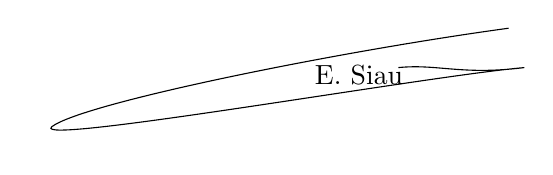
\begin{tikzpicture}[x=1cm,y=1cm]
\draw (5.8,1.25) .. controls (3.6,.95) and (.4,.3) .. (0,0) .. controls (-.3,-.25) and (4.8,.65) .. (6,.75) .. controls (5.2,.65) and (4.9,.8) .. (4.4,.75);
\node at (3.9,.65) {\unsure{E. Siau}};
\end{tikzpicture}}

\uline{E. SIAU}

\margin{137}


\scanpage{138}
$\overline{\uline{\mathrm{III}}}$\quad $\mathcal M(0)$

\diagram{\begin{tikzcd}[column sep=small,row sep=small]
\mathcal M(0) & & & \mathcal M(0)\times\mu & & & & & \\
& \mathcal M_0^! & & & \underline{\mathcal M^!}\simeq\mathcal M_0^!\times\mu & & & \mathcal M & \\
\mu_\tau & & & D_\tau & & & & & \\
& & \mathcal M^{\Pi_0}[0] & & & \mathcal M^\Pi[0]\ (\text{ou }\mathcal M^![0]) & & & \mathcal M^{\mathcal G}[0]\ \text{ou }\mathcal M[0] \\
& \Pi'_0=\mathcal G_0^! & & & \Pi'=\mathcal G^! & & & \mathcal G & \\
\{1\} & & & \underline\mu & & & & & \\
& & D_0^{\Pi_0} & & & D_0^\Pi & & & D_0^{\mathcal G} \\
& \underline\Pi_0 & & & \underline\Pi=\mathcal G^{+!} & & & \underline{\mathcal G^+} & \\
& & L_0^{\Pi_0} & & & L_0^\Pi & & & L_0^{\mathcal G}
\arrow[from=1-1,to=1-4,hook,"2"]
\arrow[from=1-1,to=2-2,hook]
\arrow[from=1-4,to=2-5,hook]
\arrow[from=2-2,to=2-5,hook,"2"]
\arrow[from=2-5,to=2-8,hook,"6"]
\arrow[from=3-1,to=1-1,hook]
\arrow[from=3-4,to=1-4,hook]
\arrow[from=3-1,to=3-4,hook,"2"]
\arrow[from=3-1,to=5-2,hook]
\arrow[from=3-4,to=5-5,hook]
\arrow[from=4-3,to=2-2,hook]
\arrow[from=4-6,to=2-5,hook]
\arrow[from=4-9,to=2-8,hook]
\arrow[from=4-3,to=4-6,hook,"2"]
\arrow[from=4-6,to=4-9,hook,"2"]
\arrow[from=5-2,to=2-2,hook]
\arrow[from=5-5,to=2-5,hook]
\arrow[from=5-8,to=2-8,hook]
\arrow[from=5-2,to=5-5,hook,"2"]
\arrow[from=5-5,to=5-8,hook,"6"]
\arrow[from=6-1,to=3-1,hook,"2"]
\arrow[from=6-1,to=6-4,hook,"2"]
\arrow[from=6-4,to=3-4,hook,"2"]
\arrow[from=6-1,to=8-2,hook]
\arrow[from=6-4,to=8-5,hook]
\arrow[from=7-3,to=4-3,hook]
\arrow[from=7-6,to=4-6,hook]
\arrow[from=7-9,to=4-9,hook]
\arrow[from=7-3,to=5-2,hook]
\arrow[from=5-2,to=7-3,bend left=7]
\arrow[from=7-6,to=5-5,hook]
\arrow[from=7-9,to=5-8,hook]
\arrow[from=7-3,to=7-6,hook,"2"]
\arrow[from=7-6,to=7-9,hook,"2"]
\arrow[from=8-2,to=5-2,hook,"2"]
\arrow[from=8-5,to=5-5,hook,"2"]
\arrow[from=8-8,to=5-8,hook,"2"]
\arrow[from=8-2,to=8-5,hook,"2"]
\arrow[from=8-5,to=8-8,hook,"6"]
\arrow[from=9-3,to=7-3,hook,"2"]
\arrow[from=9-6,to=7-6,hook,"2"]
\arrow[from=9-9,to=7-9,hook,"2"]
\arrow[from=9-3,to=8-2,hook]
\arrow[from=9-6,to=8-5,hook]
\arrow[from=9-9,to=8-8,hook]
\arrow[from=9-3,to=9-6,hook,"2"]
\arrow[from=9-6,to=9-9,hook,"2"]
\arrow[from=1-1,to=4-3,dashed,bend right=75,"\unsure{2}"']
\arrow[from=3-1,to=7-3,dashed,bend right=80]
\arrow[from=6-1,to=9-3,dashed,bend right=75]
\end{tikzcd}}

\rule{\linewidth}{0.4pt}
$\overline{\uline{\mathrm{IV}}}$\quad $Z_\rho,\ N_\rho$

\diagram{\begin{tikzcd}[column sep=small,row sep=small]
& & & Z_\rho^! & & & N_\rho & \\
\unsure{\mu_{\tau'}\cdot Z_{0\rho}^!\,\mathrm{d/m}}=\deleted{\unsure{N_{0\rho}^{?}|N_{0\rho}^!}} & & \overset{\unsure{\deleted{\mu_{\tau'}}\cdot Z_0^!\,\mathrm{d/m}}}{\unsure{N_\rho^{?}|N_\rho^!}} & & \mathcal M^! & N_\rho & & \mathcal M \\
& \unsure{Z_{0\rho}^!} & & Z_\rho^! & & & Z_\rho & \\
\mu_{\tau'} & & D_{\tau'} & & & D_\rho & & \\
& & \mathcal M_0^{\prime!} & & \mathcal M^{\prime!} & & & \mathcal M' \\
& 1 & & \mu & & & L_\rho & \\
& & \underline\Pi_0 & & \underline\Pi=\mathcal G^{+!} & & & \underline{\mathcal G^+}
\arrow[from=1-4,to=1-7,hook,"6"]
\arrow[from=1-4,to=2-5,hook]
\arrow[from=1-7,to=2-8,hook]
\arrow[from=2-1,to=2-3,hook]
\arrow[from=2-3,to=2-6,hook,dashed]
\arrow[from=2-5,to=2-8,hook,"6"]
\arrow[from=3-2,to=2-1,hook,"2"]
\arrow[from=3-4,to=2-3,hook,"2"]
\arrow[from=3-7,to=1-7,hook,"2"]
\arrow[from=3-7,to=2-6,hook,"2"]
\arrow[from=3-4,to=1-4]
\arrow[from=3-2,to=3-4,hook,"2"]
\arrow[from=3-4,to=3-7,hook,"3"]
\arrow[from=3-2,to=5-3,hook]
\arrow[from=3-4,to=5-5,hook]
\arrow[from=3-7,to=5-8,hook]
\arrow[from=4-1,to=2-1,hook]
\arrow[from=4-3,to=2-3,hook]
\arrow[from=4-6,to=2-6,hook]
\arrow[from=4-1,to=4-3,hook,dashed]
\arrow[from=4-3,to=4-6,hook,dashed]
\arrow[from=5-3,to=5-5,hook,"2"]
\arrow[from=5-5,to=5-8,hook,"6"]
\arrow[from=5-5,to=2-5,hook,"2"]
\arrow[from=5-8,to=2-8,hook,"2"]
\arrow[from=5-5,to=3-4]
\arrow[from=6-2,to=3-2,hook]
\arrow[from=6-4,to=3-4]
\arrow[from=6-7,to=3-7,hook]
\arrow[from=6-2,to=4-1,hook]
\arrow[from=6-4,to=4-3,hook]
\arrow[from=6-7,to=4-6,hook]
\arrow[from=6-2,to=6-4,hook,"2"]
\arrow[from=6-4,to=6-7,hook,"3"]
\arrow[from=6-2,to=7-3,hook]
\arrow[from=6-4,to=7-5,hook]
\arrow[from=6-7,to=7-8,hook]
\arrow[from=7-3,to=5-3,dash]
\arrow[from=7-5,to=5-5,hook]
\arrow[from=7-8,to=5-8,hook]
\arrow[from=7-3,to=7-5,hook,"2"]
\arrow[from=7-5,to=7-8,hook,"6"]
\end{tikzcd}}

\figure{\begin{tikzpicture}\draw[gray] (0,0)--(0,1.5);\draw[gray] (0,1.6)--(2,1.7);\end{tikzpicture}}
\margin{138}


\scanpage{139}
U N I V E R S I T E

DES SCIENCES ET TECHNIQUES

DU LANGUEDOC

\texttt{------------}

MONTPELLIER, le 4 Juillet 1979

Service de la Scolarité

MR / GJ

Diffusion : Liste A

N° : 3929

\uline{AVIS DE SOUTENANCE D'UNE THESE DE DOCTEUR INGENIEUR}

\uline{SCIENCES ALIMENTAIRES Option GENIE ET TECHNOLOGIE ALIMENTAIRES - FERMENTATION}

\uline{Nom et prénom du candidat} :

ARJONA José Luis

\uline{Titre de la thèse} :

``Contribution à l'étude de la torréfaction en couche fluidisée''.

\uline{Date, heure et lieu de soutenance prévus} :

\uline{11 JUILLET} 1979 à 10 Heures 30 mn

Salle de cours n° 10

U. S. T. L.

\uline{Nom du Directeur de thèse} :

Monsieur H. GIBERT

\uline{Désignation du laboratoire où la thèse est préparée} :

Génie Alimentaire.

\uline{Résumé de la thèse} :

Ce travail est centré sur l'étude d'un nouveau procédé de torréfaction mettant en oeuvre une couche fluidisée. Différentes techniques ont été essayées :

- Torréfaction par fluidisation directe des grains de café dans un courant d'air chaud,

- Torréfaction par flottation - immersion au sein d'une couche fluidisée de produits inertes portée à température adéquate.

La fluidisation s'avère un excellent moyen d'étude des mécanismes de torréfaction et de détermination des conditions opératoires optimales (température).

L'intérêt du procédé est souligné sur le plan de la consommation énergétique (très faibles durées de torréfaction), comme sur celui de la qualité des produits (uniformité de traitement de la charge).

\uline{Durée approximative des recherches ayant abouti à la thèse} : 3 ans 1/2.

\uline{Composition du jury proposé} :

MM.

GIBERT

CHARREAU

COUDERC

CROUZET

DOTHEE

VINCENT

Le Secrétaire Général,

\figure{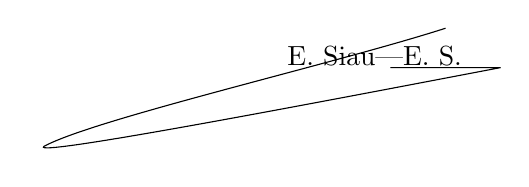
\begin{tikzpicture}[x=1cm,y=1cm]
\draw (5.1,1.5) .. controls (3.7,1.05) and (.65,.35) .. (0,0) .. controls (-.2,-.15) and (3.7,.6) .. (5.8,1.0) -- (4.4,1.0);
\node at (4.2,1.15) {\unsure{E. Siau|E. S.}};
\end{tikzpicture}}

\uline{E. S I A U}

\margin{139}


\scanpage{140}
$\overline{\uline{\mathrm{IV}}}$

\diagram{\begin{tikzcd}[column sep=small,row sep=small]
& \deleted{N_{\rho0}^{?}} & & N_\rho^{?} & & & & & \\
& & \deleted{\unsure{N_{\rho0}^{?}}} & & N_\rho^{?} & & \mathcal M^{?} & & \mathcal M \\
\mathcal M_0^{?} & & \mathcal M^{?} & & & & & & \\
& Z_{0\rho}^{!}=\unsure{\mathcal M(-\bar j)|\mathcal M(-j)} & & Z_\rho^! & & \mathcal M^{\prime!} & & \mathcal M' & \\
& \mathcal M & \mu_{\tau'} & & D_{\tau'} & & \Pi_{\tau'} & & \mathcal G \\
\mathcal M_0^{\prime!} & & \mathcal M^{\prime!} & & & & & & \\
& 1 & & \underline\mu & & \underline\Pi & & \underline{\mathcal G^+} & \\
& \mathcal M' & & & & & & & \\
\underline\Pi_0 & & \underline\Pi & & & & & & \\
& \underline{\mathcal G^+} & & & & & & &
\arrow[from=1-2,to=1-4,hook,"2"]
\arrow[from=2-3,to=2-5,hook,"2"]
\arrow[from=2-5,to=2-7,hook]
\arrow[from=2-7,to=2-9,hook,"6"]
\arrow[from=1-2,to=2-3,dashed,<->,bend left=30]
\arrow[from=1-4,to=2-5,dashed,<->,bend left=30]
\arrow[from=1-2,to=3-1,hook]
\arrow[from=1-4,to=3-3,hook]
\arrow[from=3-1,to=3-3,hook,"2"]
\arrow[from=4-2,to=1-2,hook,"2"]
\arrow[from=4-4,to=1-4,hook,"2"]
\arrow[from=4-2,to=2-3,hook,"2"]
\arrow[from=4-4,to=2-5,hook,"2"]
\arrow[from=4-6,to=2-7,hook,"2"]
\arrow[from=4-8,to=2-9,hook,"2"]
\arrow[from=4-2,to=4-4,hook,"2"]
\arrow[from=4-4,to=4-6,hook]
\arrow[from=4-6,to=4-8,hook,"6"]
\arrow[from=4-2,to=6-1,hook]
\arrow[from=4-4,to=6-3,hook]
\arrow[from=3-3,to=5-2,hook,"6"]
\arrow[from=5-2,to=4-2]
\arrow[from=5-3,to=2-3,hook]
\arrow[from=5-5,to=2-5,hook]
\arrow[from=5-7,to=2-7,hook]
\arrow[from=5-9,to=2-9,hook]
\arrow[from=5-3,to=5-5,hook,"2"]
\arrow[from=5-5,to=5-7,hook]
\arrow[from=5-7,to=5-9,hook,"6"]
\arrow[from=6-1,to=3-1,hook,"2"]
\arrow[from=6-3,to=3-3,hook,"2"]
\arrow[from=6-1,to=6-3,hook]
\arrow[from=7-2,to=5-2,hook]
\arrow[from=7-2,to=5-3,hook,"2"]
\arrow[from=7-4,to=5-5,hook,"2"]
\arrow[from=7-6,to=5-7,hook,"2"]
\arrow[from=7-8,to=5-9,hook,"2"]
\arrow[from=7-4,to=4-4,hook]
\arrow[from=7-6,to=4-6,hook]
\arrow[from=7-8,to=4-8,hook]
\arrow[from=7-2,to=7-4,hook,"2"]
\arrow[from=7-4,to=7-6,hook]
\arrow[from=7-6,to=7-8,hook,"6"]
\arrow[from=7-2,to=9-1,hook]
\arrow[from=7-4,to=9-3,hook]
\arrow[from=6-3,to=8-2,hook,"6"]
\arrow[from=8-2,to=5-2,hook,"2"]
\arrow[from=9-1,to=6-1,hook]
\arrow[from=9-3,to=6-3,hook]
\arrow[from=9-1,to=9-3,hook,"2"]
\arrow[from=9-3,to=10-2,hook,"6"]
\arrow[from=10-2,to=8-2,hook]
\arrow[from=9-3,to=7-6,<->,dashed,bend right=25]
\arrow[from=10-2,to=7-8,<->,dashed,bend right=30]
\end{tikzcd}}

\diagram{\begin{tikzcd}[color=gray,column sep=large,row sep=large]
& \unsure{\mu_{\tau'}} & & \unsure{D_{\tau'}} \arrow[rr,dash] & & \unsure{D_\rho} \\
{} \arrow[ur,dash] & & {} \arrow[ur,dash] & & &
\end{tikzcd}}

\diagram{\begin{tikzcd}[color=gray,column sep=small,row sep=small]
& \deleted{\unsure{N_{\rho0}^{?}}} & & \unsure{N_\rho^{?}} & & N_\rho & & \mathcal M \\
Z_{0\rho}^{!}=\unsure{\mathcal M(-\bar j)} & & Z_\rho^! & & Z_\rho & & \mathcal M' & \\
& \mu_{\tau'} & & D_{\tau'} & & D_\rho & & \mathcal G \\
\mathcal M_0^{\prime!} & \mathcal M^{\prime!} & & & & & & \\
& 1 & \underline\mu & & L_\rho & & \underline{\mathcal G^+} & \\
\underline\Pi_0 & \underline\Pi & & & & & &
\arrow[from=1-2,to=1-4,dash]
\arrow[from=1-4,to=1-6,dash]
\arrow[from=1-6,to=1-8,dash]
\arrow[from=2-1,to=1-2,dash]
\arrow[from=2-3,to=1-4,dash]
\arrow[from=2-5,to=1-6,dash]
\arrow[from=2-7,to=1-8,dash]
\arrow[from=2-1,to=2-3,dash]
\arrow[from=2-3,to=2-5,dash]
\arrow[from=2-5,to=2-7,dash]
\arrow[from=3-2,to=1-2,dash]
\arrow[from=3-4,to=1-4,dash]
\arrow[from=3-6,to=1-6,dash]
\arrow[from=3-8,to=1-8,dash]
\arrow[from=3-2,to=3-4,dash]
\arrow[from=3-4,to=3-6,dash]
\arrow[from=3-6,to=3-8,dash]
\arrow[from=4-1,to=2-1,dash]
\arrow[from=4-2,to=2-3,dash]
\arrow[from=4-1,to=4-2,dash]
\arrow[from=4-2,to=2-7]
\arrow[from=5-2,to=3-2,dash]
\arrow[from=5-3,to=3-4,dash]
\arrow[from=5-5,to=3-6,dash]
\arrow[from=5-7,to=3-8,dash]
\arrow[from=5-2,to=2-1,dash]
\arrow[from=5-3,to=2-3,dash]
\arrow[from=5-5,to=2-5,dash]
\arrow[from=5-7,to=2-7,dash]
\arrow[from=5-2,to=5-5,dash]
\arrow[from=5-5,to=5-7,dash]
\arrow[from=6-1,to=4-1,dash]
\arrow[from=6-2,to=4-2,dash]
\arrow[from=6-1,to=5-2,dash]
\arrow[from=6-2,to=5-3,dash]
\arrow[from=6-1,to=6-2,dash]
\arrow[from=6-2,to=5-7]
\end{tikzcd}}
\margin{140}


\scanpage{141}
\[
ST_{0,2}
\]
\[
ST_{\unsure{1,1|1,2}},\ ST_{1,2}
\]
\margin{\unsure{Au|1v}}
\margin{141}


\scanpage{142}
1) Groupe de Teichmüller spécial étendu du cylindre.

Considérons le cylindre \unsure{standart}
\[
(1)\qquad\left\{\begin{aligned}
X&=\mathbb U\times\unsure{\mathbb I|\mathbb J}\qquad\text{où}\quad \mathbb U=\{z\in\mathbb C\mid |z|=1\}\\
&&\unsure{\mathbb I|\mathbb J}=[-1,+1]
\end{aligned}\right.
\]
donc
\[
(2)\qquad \partial X=\mathbb U\times\partial\unsure{\mathbb I|\mathbb J}=\mathbb U\times\{-1,+1\}=\mathbb U_{-1}\amalg\mathbb U_1.
\]
Choisissons le revêtement universel \unsure{standart} de $\mathbb U_\varepsilon$ ($\varepsilon\in\{\pm1\}$), par
\[
(3)\qquad\left\{\begin{array}{ccc}
\inserted{\widetilde{\mathbb U}_\varepsilon\overset{\mathrm{dfn}}{=}}\mathbb R_\varepsilon&\longrightarrow&\mathbb U_\varepsilon\\
(t,\varepsilon)&\mathbin{\mapstochar\!\relbar\!\relbar\!\relbar}&(\exp(2i\pi t),\varepsilon).
\end{array}\right.
\]
Considérons le groupe ``dihédral torique''
\inserted{$(\simeq\deleted{\unsure{S}}O(2,\mathbb R))$}
\[
(4)\qquad D_{\mathbb U}\overset{\mathrm{dfn}}{=}\{1,\sigma\}\cdot\mathbb U\qquad(\tfrac12\text{ direct})
\]
où $\sigma$ est la conjugaison complexe de $\mathbb C$, opérant sur $\mathbb U$ par $z\mathbin{\mapstochar\!\relbar\!\relbar}z^{-1}$, nous choisissons comme revêtement universel de ce groupe le groupe ``dihédral réel''
\[
(5)\qquad \widetilde{D_{\mathbb U}}\overset{\mathrm{dfn}}{=}D_{\mathbb R}\overset{\mathrm{dfn}}{=}\{1,\sigma\}\cdot\mathbb R,
\]
avec l'hom de revêtement
\[
(6)\qquad \sigma^\nu\cdot t\longrightarrow\sigma^\nu\exp(2i\pi t),
\]
\margin{$\nu\in\mathbb Z/2\mathbb Z$}
de sorte qu'on a une suite exacte
\diagram{\begin{tikzcd}
(7)\quad 1 \arrow[r] & \mathbb Z \arrow[r,hook] & D_{\mathbb R} \arrow[r] & D_{\mathbb U} \arrow[r,dash] & 1.
\end{tikzcd}}
Nous faisons opérer $D_{\mathbb R}$ sur $\mathbb R_\varepsilon=\widetilde{\mathbb U}_\varepsilon$ par
\margin{142}


\scanpage{143}
\[
(8)\qquad (\sigma^\nu.u).t_\varepsilon=(-1)^\nu(t+u)_\varepsilon
\]
\margin{(NB $t_\varepsilon=(t,\varepsilon)$\quad $\varepsilon\in\{\pm1\}$)}
Cette opération passe au quotient en une opération de $D_{\mathbb R}$ sur $\deleted{\unsure{\mathbb R}}\mathbb U_\varepsilon$ et $\overline{\mathrm u}$ de $D_{\mathbb U}$ sur $\mathbb U_\varepsilon$, cette dernière est donnée par
\[
(9)\qquad (\sigma^\nu.\theta)z_\varepsilon=(z\theta)^{(-1)^\nu}=\left\{\begin{array}{ll}
z\theta&\text{si }\nu\equiv0\quad(2)\\
z^{-1}\theta^{-1}&\text{si }\nu\equiv1\quad(2).
\end{array}\right.
\]
Ainsi le groupe $D_{\mathbb R}\times D_{\mathbb R}$ opère sur
\[
\widetilde{\partial X}\overset{\mathrm{dfn}}{=}\widetilde{\mathbb U}_{-1}\amalg\widetilde{\mathbb U}_1\simeq\unsure{\widetilde{\mathbb R}_{-1}\amalg\widetilde{\mathbb R}_1},
\]
via des actions sur les deux sommandes, et cette action passe au quotient en une action de $D_{\mathbb U}\times D_{\mathbb U}$ sur $\deleted{\unsure{\partial X}}\partial X=\mathbb U_{-1}\amalg\mathbb U_1$. Nous allons prolonger cette action de $D_{\mathbb R}\times D_{\mathbb R}$ sur $\widetilde{\partial X}$ en une action sur
\[
(10)\qquad \widetilde X\overset{\mathrm{dfn}}{=}\mathbb R\times\unsure{\mathbb I|\mathbb J}
\]
qui revêt $X$ par
\[
(11)\qquad (t,s)\longmapsto(\exp2i\pi t,s)\ ;
\]
\deleted{Pour ceci} Plus exactement, c'est le sous-groupe
\[
(12)\qquad D_{\mathbb R\times\mathbb R}\overset{\mathrm{dfn}}{=}\underset{(1/2\text{ direct})}{\{1,\sigma\}.(\mathbb R\times\mathbb R)}\hookrightarrow D_{\mathbb R}\times D_{\mathbb R}
\]
\[
-\sigma^\nu.(\unsure{u_{-1}|t_{-1}},\unsure{u_1|t_1})\mathbin{\mapstochar\!\relbar\!\relbar}(\sigma^\nu.\unsure{u_{-1}|t_{-1}},\sigma^\nu.\unsure{u_{+1}|t_{+1}})
\]
qu'on va faire opérer, de façon à ce que ces opérations passent au quotient en une opération de $D_{\mathbb R\times\mathbb R}$ sur $X$ lui-$\overline{\mathrm m}$. On
\margin{143}


\scanpage{144}
désignera, pour un élément
\[
(u_{-1},u_1)\in\mathbb R^{\unsure{2}}\times\mathbb R
\]
par
\[
(13)\qquad s\longmapsto u_s
\]
l'application affine de $\mathbb R$ dans $\mathbb R$ \deleted{\unsure{def}} qui prend la valeur $u_{-1}$ pour $s=-1$, la valeur $u_1$ pour $s=+1$, \deleted{\unsure{et}} donc
\[
(14)\qquad u_s=\frac{u_1-u_{-1}}2\,s+\frac{u_1+u_{-1}}2,
\]
et on pose
\[
(15)\qquad\left\{\begin{aligned}
(u_{-1},u_1).(t,s)&\overset{\text{déf}}{=}(t+u_s,s)\\
\sigma.(t,s)&\overset{\text{déf}}{=}(-t,s)
\end{aligned}\right.
\]
d'où une opération de $D_{\mathbb R\times\mathbb R}$ sur $\widetilde X$, compatible d'ailleurs avec la \deleted{\unsure{pri}} projection
\diagram{\begin{tikzcd}
\widetilde X=\mathbb R\times\unsure{\mathbb I|\mathbb J} \arrow[r] & \unsure{\mathbb I|\mathbb J}\\
(t,s) \arrow[r,mapsto] & s
\end{tikzcd}}
et l'opération triviale sur $\unsure{\mathbb I|\mathbb J}$. L'opération passe bien au quotient en une opération de $D_{\mathbb R\times\mathbb R}$ sur $X$ lui-$\overline{\mathrm m}$, compatible avec la projection
\diagram{\begin{tikzcd}
X=\mathbb U\times\unsure{\mathbb I|\mathbb J} \arrow[r] & \unsure{\mathbb I|\mathbb J}\\
(z,\unsure{s}) \arrow[r,mapsto,no head] & s
\end{tikzcd}}
et l'opération triviale sur $\unsure{\mathbb I|\mathbb J}$.

Considérons le sous-groupe de $D_{\mathbb R\times\mathbb R}$ qui opère \unsure{trivialemt|trivialement} sur $\partial X=\mathbb U\times\{-1,+1\}$, c'est le sous-groupe $\mathbb Z\times\mathbb Z\subset D_{\mathbb R\times\mathbb R}^{0}$.
\margin{144}


\scanpage{145}
Considérons deux éléments
\[
(16)\qquad \sigma^\nu u_\cdot=\sigma^\nu.(u_{-1},u_1),\quad\sigma^{\nu'}.u'_\cdot=\sigma^{\nu'}.(u'_{-1},u'_1)
\]
de $D_{\mathbb R\times\mathbb R}$, on voit de suite qu'ils ont $\overline{\mathrm m}$ effet sur $\widetilde X$ \deleted{\unsure{et}} (et $\overline{\mathrm m}$ seulement sur $\partial\widetilde X=\widetilde{\partial X}$) ssi ils sont égaux: $D_{\mathbb R\times\mathbb R}$ opère \uline{fidèlement} sur $\widetilde X$, et $\overline{\mathrm m}$ sur $\partial\widetilde X=\widetilde{\partial X}$.

Pour que les éléments (16) aient $\overline{\mathrm m}$ action sur $X$, il f. et s. qu'on ait
\[
(17)\qquad \nu=\nu'\quad\text{et}\quad u_s-u'_s\in\mathbb Z\quad\forall s\in\unsure{\mathbb I|\mathbb J},
\]
la première condition \inserted{$\nu=\nu'$} exprimant d'ailleurs que les deux opérations envisagées ont $\overline{\mathrm m}$ effet sur l'orientation de $X$. La condition $u_s-u'_s\in\mathbb Z\quad\forall s\in\unsure{\mathbb I|\mathbb J}$ s'explicite par
\[
(18)\qquad\left\{\begin{aligned}
\frac{u_1-u_{-1}}2&=\frac{u'_1-u'_{-1}}2\qquad\text{i.e.}\quad u_1-\unsure{u_{-1}^{4}|u_{-1}}=u'_1-u'_{-1}\\
\frac{u_1+\unsure{u_{+1}|u_{-1}}}2&\equiv\frac{u'_1+u'_{-1}}2\quad(\mathbb Z)\quad\deleted{\unsure{\text{i.e. }2u_{+1}}}
\end{aligned}\right.
\]
\deleted{Ecrivons} Prenons comme paramètres, pour repérer un élément \inserted{$\sigma^\nu.(u_{-1},u_{+1})$} de $D_{\mathbb R\times\mathbb R}$, non plus ($\nu$ et) $u_{-1}$ et $u_{+1}$, mais les coeff. $a=\frac{u_1-u_{-1}}2$ et $b=\frac{u_1+u_{-1}}2$ de (14), en posant
\[
(19)\qquad f_{a,b}\overset{\text{déf}}{=}(u_{-1},u_1)\qquad\text{avec}\quad\begin{aligned}u_{-1}&=-a+b\\u_1&=a+b\end{aligned}
\]
Alors on trouve
\[
(20)\qquad\deleted{\unsure{f}}f_{a,b}=f_{a',b'}\Longleftrightarrow a=a',\ b\equiv b'\ (\mathbb Z)
\]
\margin{145}


\scanpage{146}
Ainsi, le groupe quotient de $D_{\mathbb R\times\mathbb R}$ qui opère fidèlement sur $X$ est le groupe
\[
(21)\qquad D_{\mathbb R\times\mathbb U}\overset{\mathrm{dfn}}{=}\{1,\sigma\}.(\mathbb R\times\mathbb U)\qquad(1/2\text{ direct})
\]
où $\sigma$ opère \inserted{encore} sur $\mathbb R\times\mathbb U$ par symétrie
\[
\sigma(u,\theta)=(-u,\theta^{-1}).
\]
On fait opérer \deleted{\unsure{ce}} \inserted{$D_{\mathbb R\times\mathbb U}$} sur $X$ par
\[
(22)\qquad\left\{\begin{aligned}
\sigma(z,s)&=(z^{-1},s)\\
g_{\underset{\substack{\rotatebox{90}{$\in$}\\\mathbb R}}{a},\underset{\substack{\rotatebox{90}{$\in$}\\\mathbb U}}{\theta}}(z,s)&\overset{\text{déf}}{=}(z\exp(2i\pi as)\theta,s)
\end{aligned}\right.
\]
et cette action se relève en une action de $D_{\mathbb R\times\mathbb R}$ sur $\widetilde X$ par
\[
(23)\qquad\left\{\begin{aligned}
\sigma(t,s)&\overset{\text{déf}}{=}(-t,s)\\
f_{\underset{\substack{\rotatebox{90}{$\in$}\\\mathbb R}}{a},\underset{\substack{\rotatebox{90}{$\in$}\\\mathbb R}}{b}}(t,s)&\overset{\text{déf}}{=}(t+(as+b),s)
\end{aligned}\right.
\]
\deleted{Considérons} On fera opérer le groupe
\[
(24)\qquad\{\pm1\}\unsure{\ltimes|\times}D_{\mathbb R\times\mathbb U}
\]
\margin{(1/2 direct, via op. de $\pm1$ sur $D_{\mathbb R\times\mathbb U}$ par chgt de signe sur le facteur $\mathbb R$}
sur $X$, par
\[
(2\unsure{5|4})\qquad (\varepsilon\times\sigma^\nu.g_{a,\theta})(z,s)\overset{\text{déf}}{=}\left((z^{\deleted{\unsure{-1}}}\exp(2i\pi as)\theta)^{(-1)^\nu},\varepsilon s\right)
\]
cette opération se relève en une op. de
\[
(26)\qquad\{\pm1\}\unsure{\ltimes|\times}D_{\mathbb R\times\mathbb R}
\]
\margin{(1/2 direct, via op. de $\pm1$ sur $D_{\mathbb R\times\mathbb R}$ par chgt de signe sur le facteur $a$ de $f_{a,b}$ ...)}
sur $\widetilde X$, par
\[
(27)\qquad (\varepsilon\times\sigma^\nu f_{\underset{\substack{\rotatebox{90}{$\in$}\\\mathbb R}}{a},\underset{\substack{\rotatebox{90}{$\in$}\\\mathbb R}}{b}})(t,s)\overset{\text{déf}}{=}\left((\unsure{-1|+1})^\nu(t+(as+b)),\unsure{\varepsilon}s\right)
\]
\margin{146}


\scanpage{147}
Considérons le sous-groupe de \deleted{\unsure{ce}} $D_{\mathbb R\times\mathbb U}$ formé des $f_{a,\theta}$ qui \deleted{ont} sur $(\partial X)_{-1}$ et $(\partial X)_{+1}$ sont des \deleted{\unsure{auto}} op. d'ordre fini, ce qui s'exprime par les conditions
\[
\theta\exp-2i\pi a,\quad\theta\exp2i\pi a\quad\in\deleted{\unsure{\infty}}\mu_\infty(\mathbb C)
\]
\margin{(ens. des él. d'ordre fini de $\mathbb U$)}
soit encore
\[
(28)\qquad\theta\in\mu_\infty(\mathbb C),\quad a\in\mathbb Q.
\]
Ce sous-groupe est stable par l'opération de $\{\pm1\}\times\{1,\sigma\}$, opérant de la façon explicitée plus haut -- donc on trouve un ss-groupe de (24), formé \inserted{justement} par les opérations \inserted{(\unsure{dudit gr|du total gr}} qui sur $\partial X$ sont d'ordre fini. Ce sous-groupe \deleted{est} s'identifie :
\[
(29)\qquad G=\deleted{\unsure{\{\pm1\}\ltimes}}(\mu\times\mu).(\mathbb Q\times\mu_\infty)\qquad1/2\text{ direct}
\]
où $\mu=\{\pm1\}$, $\mu_\infty=\mu_\infty(\mathbb C)\simeq\mathbb Q/\mathbb Z$
\[
\exp2i\pi q\longleftarrow\!\shortmid\ q\bmod\mathbb Z
\]
et où $\mu\times\mu$ opère sur $\mathbb Q\times\mu_\infty$ par symétrie sur les deux facteurs. On identifie bien sûr $\sigma$ à $(-1,-1)\in\mu\times\mu$. On pose
\[
(30)\qquad\deleted{\unsure{G}}\widetilde G=(\mu\times\mu).(\mathbb Q\times\mathbb Q)\qquad1/2\text{ direct}
\]
avec une suite exacte
\diagram{\begin{tikzcd}
(31)\quad 1 \arrow[r,dash] & \mathbb Z \arrow[r] & \deleted{\unsure{G}}\widetilde G \arrow[r] & G \arrow[r] & 1\\
& n \arrow[r,mapsto] & \unsure{\{f_{1,n}\}|f_{0,n}} & & \\
& & (\varepsilon,\varepsilon').\unsure{\{f_{a,b}\}|f_{a,b}} \arrow[r,mapsto] & (\varepsilon,\varepsilon').\unsure{\{g_{a,\exp2i\pi b}\}|g_{a,\exp2i\pi b}} &
\end{tikzcd}}
\margin{147}


\scanpage{148}
L'opération de $\deleted{\unsure{G}}\widetilde G$ sur $\widetilde X$ est donnée par
\margin{$\deleted{\unsure{(\varepsilon,\varepsilon')=(\varepsilon',\varepsilon\varepsilon')}}$}
\[
(\unsure{32|31})\quad\left((\underset{\substack{\rotatebox{90}{$\in$}\\\mu}}\varepsilon,\underset{\substack{\rotatebox{90}{$\in$}\\\mu}}{\varepsilon'}).f_{\underset{\substack{\rotatebox{90}{$\in$}\\\mathbb Q}}a,\underset{\substack{\rotatebox{90}{$\in$}\\\mathbb Q}}b}\right)(\underset{\substack{\rotatebox{90}{$\in$}\\\mathbb R}}t,\underset{\substack{\rotatebox{90}{$\in$}\\\unsure{\mathbb I|\mathbb J}}}s)
=(\varepsilon'(t+(as+b)),\varepsilon\varepsilon's)=\varepsilon'(t+(as+b),\varepsilon s)
\]
elle passe aux quotients en l'action de $G$ sur $X$
\[
(33)\quad\left((\underset{\substack{\rotatebox{90}{$\in$}\\\mu}}\varepsilon,\underset{\substack{\rotatebox{90}{$\in$}\\\mu}}{\varepsilon'}).g_{\underset{\substack{\rotatebox{90}{$\in$}\\\mathbb Q}}a,\underset{\substack{\rotatebox{90}{$\in$}\\\mu_\infty}}\theta}\right)(z,s)=\left((z\theta\exp2i\pi as)^{\varepsilon'},\varepsilon\varepsilon's\right).
\]
Pour l'opération $(\varepsilon,\varepsilon').g_{a,\unsure{b|s}}$, $\varepsilon$ est le caractère d'orientation (l'orientation conservée ou non suivant que $\varepsilon=+1$ ou $\varepsilon=-1$), $\varepsilon\varepsilon'$ est le signe qui indique l'action sur $\pi_0(\partial X)$ (``ensemble des trous''). L'action de $G$ sur $\partial X$ s'obtient essentiellement, le signe $\varepsilon\varepsilon'$ pris, \deleted{\unsure{par les}} indiquant s'il y a transposition entre les deux comp. connexes, \deleted{\unsure{par les}} et un signe $\varepsilon'$ pris indiquant s'il faut composer avec une conjugaison complexe, par les deux rotations $\theta\exp(-2i\pi a),\ \theta\exp(2i\pi a)$.

\deleted{Exprimons que l'on a
\[
(34)\qquad\theta\exp-2i\pi a=-1\qquad\theta\exp2i\pi a=-1
\]
on trouve les deux \inserted{types de} solutions
\[
(35)\qquad\begin{aligned}
\theta&=1& a&\in\tfrac12+\mathbb Z\\
\theta&=-1& a&\in\mathbb Z
\end{aligned}
\]}
\margin{148}


\scanpage{149}
\deleted{ou plus simplement, si $\theta=\exp2i\pi b$, en termes de $a$ et $b$
\[
(36)\qquad\left\{\begin{array}{rcll}
&\smash{\raisebox{-1ex}{$\Big\{$}}&a\equiv\tfrac12,&b\equiv1\quad(\mathbb Z)\\
\text{ou}&&a\equiv1,&b\equiv\tfrac12\quad(\mathbb Z)
\end{array}\right.
\]
Nous nous intéressons plus particulièrement au sous-groupe}

Nous nous intéressons au sous-groupe $G_0$ de $G$ correspondant à la valeur $\theta=1$, on écrira $g_a$ au lieu de $g_{a,\theta}$, donc
\[
(34)\qquad g_a(\unsure{z},s)=(z\exp2i\pi\unsure{as},s)
\]
Pour que cette opération induise l'identité sur $\partial X$, il f. et s. qu'on ait
\[
(35)\qquad\exp2i\pi a=1\qquad\text{i.e.}\quad a\in\mathbb Z.
\]
Nous nous intéressons au sous-groupe
\margin{149}


\scanpage{150}
\uline{Cylindre}\quad\deleted{\unsure{de}} $X$

trois ensembles à 2 éléments
\diagram{\[\begin{array}{ll|l}
a)&\pi_0\partial X&\varepsilon_0(X)\\
b)&\text{ens des deux générateurs de }\pi_1(X)\simeq H_1(X)&\varepsilon_1(X)\\
c)&\text{ens des deux orientations de }X&\omega(X)
\end{array}\]}
On a un iso. canonique
\[
\omega(X)\simeq\varepsilon_0(X)\wedge\varepsilon_1(X)
\]
Si on a une comp. \inserted{$S$} du bord ($\alpha\in\varepsilon_0(X)$) et une orientation du bord ($\beta\in\varepsilon_1(X)=\text{ens des deux génér. de }H_1(S)$) on a une orientation de $X$: celle qui induit $\beta$ sur $\alpha$ ...

\margin{\figure{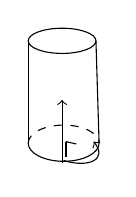
\begin{tikzpicture}[x=1cm,y=1cm]
\draw (0,0) ellipse (.43 and .16);
\draw (-.43,0)--(-.43,-1.3);\draw (.43,0)--(.47,-1.3);
\draw (-.43,-1.3) arc[start angle=180,end angle=360,x radius=.45,y radius=.23];
\draw[dashed] (-.43,-1.3) arc[start angle=180,end angle=0,x radius=.45,y radius=.23];
\draw[->] (0,-1.55)--(0,-.75);
\draw[->] (.02,-1.52) .. controls (.35,-1.62) and (.58,-1.5) .. (.4,-1.28);
\draw (.05,-1.28)--(.05,-1.48);\draw (.05,-1.28)--(.18,-1.31);
\end{tikzpicture}}}
Soit un autom \inserted{$u$} de $\unsure{\alpha|X}$ induisant l'identité sur $\partial X$. Il peut se relever en un autom. de $\widetilde X$ unique \inserted{$\widetilde u^{(S)}$} induisant l'identité sur $\widetilde X|S$ -- Alors son action sur $\widetilde X|S'$ est \deleted{\unsure{une}} \inserted{induite} par un élément \deleted{de} $n\in H_1(S')\xleftarrow{\sim}H_1(X)$. Si on \deleted{change} \inserted{remplace} $S$ par $S'$, on trouve $\widetilde u^{(S')}$, \deleted{\unsure{qui}}
\margin{$S'=\partial X\setminus S$}
\[
\widetilde u^{S'}=\tau_n^{-1}\widetilde u^S=\tau_{-n}\widetilde u^S
\]
\deleted{de} \unsure{qui|que} restreint à $S$ donne $\tau_{-n}$. Donc il y a un invariant qui est dans
\[
\begin{aligned}
H_1(X)\wedge_{\{\pm1\}}\varepsilon_0(X)
&=(\mathbb Z\wedge_{\pm1}\unsure{\varepsilon_0(X)|\varepsilon_1(X)})\wedge_{\pm1}\varepsilon_0(X)\\
&\simeq\mathbb Z\wedge_{\pm1}(\varepsilon_1(X)\wedge\varepsilon_0(X))\\
&\simeq\mathbb Z\wedge_{\pm1}\omega(X)
\end{aligned}
\]
\margin{150}


\scanpage{151}
UNIVERSITE\\
DES SCIENCES ET TECHNIQUES\\
DU LANGUEDOC\\
------------

MONTPELLIER, le 17 Septembre 1980

Service de la Scolarité\\
MA/GJ\\
Diffusion : Liste A\\
N° : 4660

\uline{AVIS DE SOUTENANCE D'UNE THESE DE DOCTORAT DE 3ème CYCLE}

\uline{ENDOCRINOLOGIE}

\uline{Nom et prénom du candidat} : VIC Patrice

\uline{Titre de la thèse} : MODIFICATIONS ULTRASTRUCTURALES PRECOCES DE LA CHROMATINE INDUITES \uline{PAR LES OESTROGENES} DANS LES CELLULES EPITHELIALES DE L'UTERUS ET DES TUMEURS MAMMAIRES.

\uline{Date, heure et lieu de soutenance} : 6 OCTOBRE 1980 à 10 Heures\\
Salle de cours n° 9 - USTL

\uline{Nom du Directeur de thèse} : M. ROCHEFORT H.

\uline{Désignation du laboratoire où la thèse est préparée} : INSERMU 148 - Laboratoire d'endocrinologie moléculaire et cellulaire.

\uline{Résumé de la thèse} :

L'oestradiol transforme \uline{in vitro} et \uline{in vivo} en 60 min la chromatine condensée en chromatine dispersée. Ces modifications sont observées dans l'endomètre d'agnelle et de ratte impubères et dans les tumeurs mammaires hormono-dépendantes induites par le 7,12 Dimethylbenzanthracène, mais pas dans les tumeurs mammaires C3H hormonoindépendantes de souris. La DHT à dose pharmacologique a le même effet que l'oestradiol, alors que des hormones n'ayant pas d'affinité pour les récepteurs oestrogènes sont sans effet ; les antioestrogènes, comme le tamoxifène, provoquent à l'opposé une hypercondensation de la chromatine. Dans l'endomètre d'agnelle, cette décondensation de la chromatine serait une conséquence très rapidede la stimulation de la transcription. Ces résultats suggèrent sur le plan fondamental\unsure{:}que cette décondensation de la chromatine globale et précoce, serait due à une activité de nombreux gènes. Sur un plan pratique, ces observations pourraient constituer un test morphologique de prédiction de l'hormonodépendance dans les cancers du sein humain qui pourrait compléter le dosage des récepteurs hormonaux.

\uline{Durée approximative des recherches ayant abouti à la thèse} : 3 ans

\uline{Composition du jury proposé} :\\
MM. ASSENMACHER I.\\
SENTEIN P.\\
ROCHEFORT H.\\
Mme VIGNON F.

Pour le Secrétaire Général\\
L'Attachée d'Administration Universitaire

\figure{
\begin{tikzpicture}[x=1cm,y=1cm]
\draw (0,0) .. controls (-.08,.25) and (.28,.55) .. (.20,.72) .. controls (.12,.82) and (.02,.35) .. (.08,.15) .. controls (.18,.02) and (.15,.38) .. (.02,.37) .. controls (-.08,.28) and (.03,.01) .. (.04,-.04);
\end{tikzpicture}}
\uline{\unsure{Gentil}}\\
\uline{A. GENTIL}

\margin{151}


\scanpage{152}
\margin{152}


\scanpage{153}
\texttt{//*\quad GUTS\quad 0037\qquad 1}

\diagram{\[\begin{array}{@{}llll@{}}
\mathtt{\phantom{G}GGGGGGGGGG\phantom{G}} & \mathtt{UU\phantom{UUUUUUUU}UU} & \mathtt{TTTTTTTTTTTT} & \mathtt{\phantom{S}SSSSSSSSSS\phantom{S}}\\
\mathtt{GGGGGGGGGGGG} & \mathtt{UU\phantom{UUUUUUUU}UU} & \mathtt{TTTTTTTTTTTT} & \mathtt{SSSSSSSSSSSS}\\
\mathtt{GG\phantom{GGGGGGGG}GG} & \mathtt{UU\phantom{UUUUUUUU}UU} & \mathtt{\phantom{TTTTT}TT\phantom{TTTTT}} & \mathtt{SS\phantom{SSSSSSSS}SS}\\
\mathtt{GG\phantom{GGGGGGGGGG}} & \mathtt{UU\phantom{UUUUUUUU}UU} & \mathtt{\phantom{TTTTT}TT\phantom{TTTTT}} & \mathtt{SS\phantom{SSSSSSSSSS}}\\
\mathtt{GG\phantom{GGGGGGGGGG}} & \mathtt{UU\phantom{UUUUUUUU}UU} & \mathtt{\phantom{TTTTT}TT\phantom{TTTTT}} & \mathtt{SSS\phantom{SSSSSSSSS}}\\
\mathtt{GG\phantom{GGGGGGGGGG}} & \mathtt{UU\phantom{UUUUUUUU}UU} & \mathtt{\phantom{TTTTT}TT\phantom{TTTTT}} & \mathtt{\phantom{S}SSSSSSSSS\phantom{SS}}\\
\mathtt{GG\phantom{GGGGG}GGGGG} & \mathtt{UU\phantom{UUUUUUUU}UU} & \mathtt{\phantom{TTTTT}TT\phantom{TTTTT}} & \mathtt{\phantom{SS}SSSSSSSSS\phantom{S}}\\
\mathtt{GG\phantom{GGGGG}GGGGG} & \mathtt{UU\phantom{UUUUUUUU}UU} & \mathtt{\phantom{TTTTT}TT\phantom{TTTTT}} & \mathtt{\phantom{SSSSSSSSS}SSS}\\
\mathtt{GG\phantom{GGGGGGGG}GG} & \mathtt{UU\phantom{UUUUUUUU}UU} & \mathtt{\phantom{TTTTT}TT\phantom{TTTTT}} & \mathtt{\phantom{SSSSSSSSSS}SS}\\
\mathtt{GG\phantom{GGGGGGGG}GG} & \mathtt{UU\phantom{UUUUUUUU}UU} & \mathtt{\phantom{TTTTT}TT\phantom{TTTTT}} & \mathtt{SS\phantom{SSSSSSSS}SS}\\
\mathtt{GGGGGGGGGGGG} & \mathtt{UUUUUUUUUUUU} & \mathtt{\phantom{TTTTT}TT\phantom{TTTTT}} & \mathtt{SSSSSSSSSSSS}\\
\mathtt{\phantom{G}GGGGGGGGGG\phantom{G}} & \mathtt{\phantom{U}UUUUUUUUUU\phantom{U}} & \mathtt{\phantom{TTTTT}TT\phantom{TTTTT}} & \mathtt{\phantom{S}SSSSSSSSSS\phantom{S}}
\end{array}\]}

\begin{tabular}{@{}l@{}}
\texttt{****P\quad END\quad STC\quad 37\quad GUTS\qquad ROOM\quad 11.42.58 AM 06 NOV 82\quad R6.PR1\quad SYS JES2\quad STC\quad 37\quad END\quad P****}\\
\texttt{****P\quad END\quad STC\quad 37\quad GUTS\qquad ROOM\quad 11.42.58 AM 06 NOV 82\quad R6.PR1\quad SYS JES2\quad STC\quad 37\quad END\quad P****}\\
\texttt{****P\quad END\quad STC\quad 37\quad GUTS\qquad ROOM\quad 11.42.58 AM 06 NOV 82\quad R6.PR1\quad SYS JES2\quad STC\quad 37\quad END\quad P****}\\
\texttt{****P\quad END\quad STC\quad 37\quad GUTS\qquad ROOM\quad 11.42.58 AM 06 NOV 82\quad R6.PR1\quad SYS JES2\quad STC\quad 37\quad END\quad P****}\\
\texttt{****P\quad END\quad STC\quad 37\quad GUTS\qquad ROOM\quad 11.42.58 AM 06 NOV 82\quad R6.PR1\quad SYS JES2\quad STC\quad 37\quad END\quad P****}\\
\texttt{****P\quad END\quad STC\quad 37\quad GUTS\qquad ROOM\quad 11.42.58 AM 06 NOV 82\quad R6.PR1\quad SYS JES2\quad STC\quad 37\quad END\quad P****}
\end{tabular}

\margin{153}


\scanpage{154}
\[
\deleted{\widetilde\rho^{3}(\widetilde\tau'_\infty)
=\widetilde\omega_0^{-1}\widetilde\tau'_\infty\widetilde\omega_0
=\widetilde\omega_0^{-1}\underbrace{\widetilde\tau'_\infty\widetilde\omega_0\widetilde\tau_\infty^{\prime-1}}\widetilde\tau'_\infty
=\widetilde\omega_0^{-2}\widetilde\tau'_\infty
=\ell_0^{\prime-1}\widetilde\tau'_\infty}
\]
\[
\tau'',\ \tau,\ \unsure{\varepsilon|\xi}_0,\ \unsure{\varepsilon|\xi}_1,\ \unsure{\varepsilon|\xi}_2
\]
\diagram{\[\begin{array}{lll}
\tau'',\unsure{\varepsilon|\xi}_0,\unsure{\varepsilon|\xi}_1 & \deleted{\unsure{engendrent}}\ \text{engendrent} & Gl(2,\mathbb Z)\Bigg]\ \tau\ \text{permute}\\
\tau'',\unsure{\varepsilon|\xi}_2,\unsure{\varepsilon|\xi}_1^{-1} & \rule{4cm}{.4pt} & Gl(2,\mathbb Z)\qquad\text{ces deux ss-}\\
\tau'',\unsure{\varepsilon|\xi}_1 & \rule{4cm}{.4pt} & D_{\deleted{\infty}\unsure{\varepsilon|\xi}_1}\qquad\text{groupes }Gl(2,\mathbb Z)
\end{array}\]}
\margin{et opère $-1$ sur $D_{\unsure{\varepsilon|\xi}_1}$}
\[
\mathcal T^!_{1,2}\ \overset{?}{\overset{\sim}{\longleftarrow}}\ Gl(2,\mathbb Z)*_{D_\infty}Gl(2,\mathbb Z)
\]

\figure{\begin{tikzpicture}[x=1cm,y=1cm]
\draw (-2.6,-.2) .. controls (-2.8,1.5) and (-1.8,3.1) .. (-.5,3.35) .. controls (1.5,4.05) and (2.7,2.1) .. (2.55,-.5);
\draw (-2.65,-.35) .. controls (-2.6,-1.65) and (-1.5,-2.65) .. (-.2,-2.75) .. controls (.8,-2.9) and (1.25,-2.55) .. (1.35,-2.4);
\draw (1.48,-2.28) .. controls (2.05,-1.95) and (2.38,-1.4) .. (2.45,-.85);
\draw (-.16,3.4) .. controls (-.7,2.65) and (-.88,1.1) .. (-.99,.08) -- (-.94,.02) -- (-.93,.2);
\draw (.33,3.28) .. controls (-.1,2.55) and (-.34,1.3) .. (-.37,.06);
\draw (.58,3.16) .. controls (.8,2.95) and (.78,1.3) .. (.97,.36);
\draw (.93,3.34) .. controls (1.2,2.45) and (1.45,1.15) .. (1.55,.42);
\draw (-2.32,1.85) -- (-1.8,2.48) -- (-1.8,2.35);
\end{tikzpicture}}

$3g$ cylindres qui sont deux à deux en posit°, standart (deux cylindres polaires $\equiv$ pôle, ou un cylindre polaire et un transverse relatif $\unsure{\leftrightarrow|\longrightarrow}\ \equiv$ axe équatorial) ou ne se rencontrent pas.
\[
2g+2\,\frac{g(g-1)}2=2g\left(1+\frac{g-1}2\right. =2\,\frac{g(g+1)}2
\]
paires de cylindres en position ``standart'', et les autres paires sont disjointes

MR LE PROFESSEUR GROTHENDIECK ALEX. D\\
MATHEMATIQUES\qquad 5

\margin{154}


\scanpage{155}
UNIVERSITÉ DES SCIENCES ET TECHNIQUES\\
DU LANGUEDOC\\
----

Service du Personnel\\
Diffusion liste D + affichage\\
N° 4782

\uline{ACCES DES VEHICULES AUTOMOBILES}\\
\uline{SUR LE CAMPUS DE L'U.S.T.L.}\\
--------

Je vous rappelle que l'accès des véhicules automobiles sur le campus est réservé aux détenteurs d'un coupe-file.

Ceux-ci sont délivrés par le service du Personnel (bureau d'accueil) :

-- soit à titre définitif (macarons plastifiés auto-collants) pour les personnels permanents d'Enseignement, Administratifs, Techniques et de Service.

-- soit sous forme de laissez-passer provisoires (bristol vert) valables pour l'année universitaire. Ces derniers peuvent être délivrés :

\[
\left.\begin{array}{l}
\text{-- aux personnels du C.N.R.S.}\\
\text{-- aux personnels sous convention}
\end{array}\right\}
\begin{array}{l}
\text{au vu d'une attestation du Chef de}\\
\text{Service et de la carte grise du}\\
\text{véhicule}
\end{array}
\]

-- aux thésards d'Etat et de 3ème cycle, au vu d'un certificat de scolarité et de la carte grise du véhicule.

La validité des laissez-passer provisoires délivrés au titre de l'année universitaire 1979 - 1980 expirant le \uline{31 Octobre 1980,} les détenteurs de ces cartes sont invités à se présenter au Service du Personnel (bureau d'accueil) munis des pièces mentionnées ci-dessus, pour retirer les nouveaux laissez-passer valables pour l'année universitaire 1980 -- 1981.

Le Président,

L. Thaler\\
L. THALER

\figure{
\begin{tikzpicture}[x=1cm,y=1cm]
\draw (15:1.55) arc[start angle=15,end angle=-298,radius=1.55];
\draw (15:1.16) arc[start angle=15,end angle=-291,radius=1.16];
\node[rotate=48] at (-1.05,.95) {\unsure{PRÉSIDENCE}};
\node[rotate=42] at (.65,-1.12) {\unsure{MONTPELLIER}};
\node[rotate=-22,align=center,font=\small] at (0,0) {\unsure{UNIVERSITÉ}\\\unsure{DES}\\SCIENCES et \unsure{TECHNIQUES}\\\unsure{DU}\\LANGUEDOC};
\end{tikzpicture}}

\margin{155}


\scanpage{156}
\figure{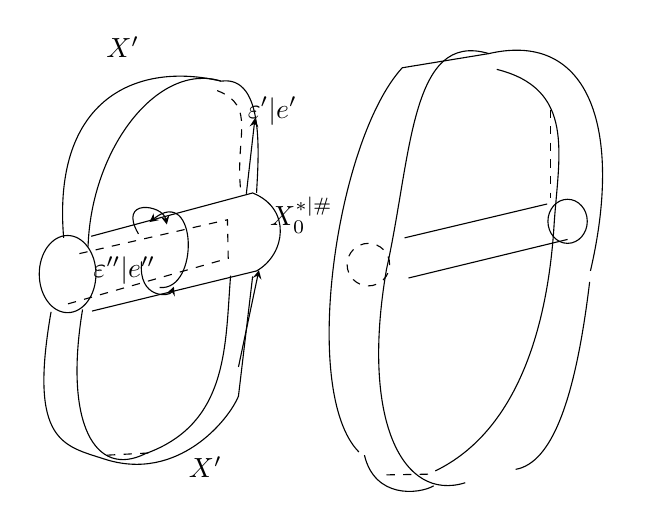
\begin{tikzpicture}[x=1cm,y=1cm,>=stealth]
\draw (-2.65,0) ellipse (.36 and .49);
\draw (-2.7,.46) .. controls (-2.85,2.25) and (-1.75,2.7) .. (-.7,2.45) .. controls (-.13,2.53) and (-.23,1.45) .. (-.25,1.03);
\draw (-2.39,.35) .. controls (-2.35,1.6) and (-1.5,2.7) .. (-.7,2.45);
\draw (-2.86,-.48) .. controls (-3.15,-2.14) and (-2.7,-2.18) .. (-2.18,-2.35) .. controls (-1.25,-2.65) and (-.6,-1.85) .. (-.48,-1.55) -- (-.3,-.03);
\draw (-2.46,-.45) .. controls (-2.7,-1.9) and (-2.3,-2.6) .. (-1.66,-2.28) .. controls (-.6,-1.9) and (-.65,-.9) .. (-.58,-.02);
\draw (-2.35,.48) -- (-.3,1.03) .. controls (.2,.83) and (.12,.25) .. (-.25,.04) -- (-2.34,-.47);
\draw[dashed] (-2.5,.26) -- (-.62,.69) -- (-.61,.2) -- (-2.65,-.38);
\draw[->] (-1.48,-.17) .. controls (-.97,-.22) and (-1,1.14) .. (-1.61,.66);
\draw[->] (-1.75,.51) .. controls (-2.02,.97) and (-1.44,.88) .. (-1.39,.63);
\draw[->] (-1.71,.16) .. controls (-1.76,-.32) and (-1.35,-.29) .. (-1.3,-.16);
\draw[->] (-.48,-1.18) -- (-.22,.05);
\draw[->] (-.38,1.02) -- (-.27,1.98);
\draw[dashed] (-.75,2.33) .. controls (-.24,2.13) and (-.53,1.75) .. (-.45,1.05);
\draw[dashed] (-2.15,-2.3) -- (-1.58,-2.27);
\node at (-1.95,2.88) {$X'$}; \node at (-.9,-2.45) {$X'$};
\node at (.32,.75) {$X_0^{\unsure{*|\#}}$};
\node at (-.05,2.07) {$\unsure{\varepsilon'|e'}$}; \node at (-1.93,.05) {$\unsure{\varepsilon''|e''}$};
\draw (1.05,-2.26) .. controls (.3,-1.5) and (.76,1.7) .. (1.6,2.62) -- (2.7,2.8) .. controls (4,3.1) and (4.4,1.8) .. (3.99,.04);
\draw (2.7,2.8) .. controls (1.7,3.1) and (1.72,1.5) .. (1.4,.06) .. controls (1.07,-1.85) and (1.6,-2.9) .. (2.4,-2.65);
\draw (1.12,-2.3) .. controls (1.25,-2.85) and (1.8,-2.8) .. (2,-2.69);
\draw (2.8,2.6) .. controls (3.8,2.35) and (3.59,1.53) .. (3.53,.65) .. controls (3.45,-.7) and (3.05,-2) .. (2.02,-2.5);
\draw (3.98,-.1) .. controls (3.8,-1.6) and (3.5,-2.4) .. (3.04,-2.48);
\draw (1.63,.46) -- (3.44,.89); \draw (1.68,-.05) -- (3.7,.44);
\draw (3.7,.67) ellipse (.25 and .28);
\draw[dashed] (1.17,.12) ellipse (.27 and .27);
\draw[dashed] (1.4,-2.55) -- (2.01,-2.54);
\draw[dashed] (3.48,2.09) -- (3.48,.97);
\end{tikzpicture}}

\[
\begin{array}{lll}
\tau' & \tau'' & \tau^{\deleted{\unsure{'''}}}\\
\unsure{\varepsilon'|\rho'} & \varepsilon^{\deleted{\unsure{''}}} & \overline\varepsilon'
\end{array}
\]

\figure{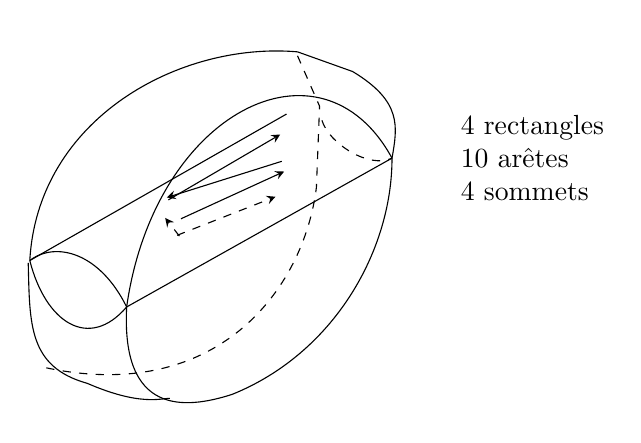
\begin{tikzpicture}[x=1cm,y=1cm,>=stealth]
\draw (-2.3,-.55) .. controls (-2.2,1.25) and (-.4,2.23) .. (1.1,2.1) -- (1.8,1.85) .. controls (2.43,1.47) and (2.37,1.15) .. (2.3,.75);
\draw (-2.32,-.58) .. controls (-2.3,-1.36) and (-2.32,-1.9) .. (-1.57,-2.11) .. controls (-.9,-2.4) and (-.64,-2.3) .. (-.52,-2.3);
\draw (-1.07,-1.14) .. controls (-1.14,-2.5) and (-.35,-2.45) .. (.27,-2.25) .. controls (1.56,-1.73) and (2.3,-.43) .. (2.3,.75);
\draw (-1.07,-1.14) .. controls (-.72,1.34) and (1.4,2.4) .. (2.3,.75);
\draw (-2.3,-.55) .. controls (-1.97,-.3) and (-1.41,-.45) .. (-1.07,-1.14) .. controls (-1.55,-1.7) and (-2.1,-1.34) .. (-2.3,-.55);
\draw (-2.3,-.55) -- (.96,1.31); \draw (-1.07,-1.14) -- (2.3,.75);
\draw[dashed] (1.1,2.05) -- (1.38,1.41) -- (1.34,.38) .. controls (1.18,-.92) and (.07,-2.4) .. (-2.15,-1.9);
\draw[dashed] (1.41,1.23) .. controls (1.5,.93) and (2.02,.61) .. (2.3,.75);
\draw[->] (-.54,.22) -- (.88,1.05); \draw[->] (.9,.71) -- (-.56,.25);
\draw[->] (-.38,-.02) -- (.93,.58); \draw[->,dashed] (-.43,-.23) -- (.82,.26);
\draw[->,dashed] (-.4,-.24) -- (-.58,-.01);
\node[anchor=west,align=left] at (3.05,.75) {4 rectangles\\10 arêtes\\4 sommets};
\end{tikzpicture}}

\figure{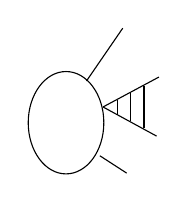
\begin{tikzpicture}[x=1cm,y=1cm]
\draw (0,0) ellipse (.48 and .65);
\draw (.26,.53)--(.72,1.2); \draw (.43,-.42)--(.77,-.64);
\draw (.47,.2)--(1.18,.58); \draw (.47,.2)--(1.15,-.17);
\draw (.65,.1)--(.65,.29); \draw (.82,.02)--(.82,.38); \draw (.99,-.07)--(.99,.47);
\end{tikzpicture}}
\[
\tau^{\prime2}=\tau^{\prime\prime2}=\tau^2
=\deleted{\unsure{(\tau''\tau)^2=\tau\tau''=\tau''\tau'}};
(\tau''\tau)^2=(\tau\tau')^2=(\tau'\tau'')^2=1
\]
\[
\begin{aligned}
\tau(\varepsilon_0)&=\varepsilon_2\qquad(\tau(\varepsilon_2)=\unsure{\tau(\varepsilon_1)|\tau(\varepsilon_0)} )\\
\tau(\varepsilon_1)&=\varepsilon_1^{-1}\\
\tau'(\varepsilon_0)&=\tau''(\varepsilon_0)=\varepsilon_0^{-1}\\
\bigl(\Rightarrow\quad\tau'(\varepsilon_{\unsure{1|2}})&=\tau''(\varepsilon_2)=\varepsilon_2^{-1}\bigr)\\
\tau'(\varepsilon_1)&=\tau''(\varepsilon_1)=\varepsilon_1^{-1}\\
[\varepsilon_0,\varepsilon_2]&=1
\end{aligned}
\]
\margin{$\begin{aligned}
\rho_0&\overset{\mathrm{dfn}}=(\varepsilon_1\varepsilon_0)^{-1}=\varepsilon_0^{-1}\varepsilon_1^{-1}\\
\tau(\rho_0)&=(\varepsilon_1^{-1}\varepsilon_2)^{-1}\overset{\mathrm{dfn}}=\rho_2\\
&=\varepsilon_2^{-1}\varepsilon_1\\
\Rightarrow\quad(\underbrace{\varepsilon_1\varepsilon_0}_{\rho_0^{-1}})^3
&=(\underbrace{\varepsilon_0\varepsilon_1\varepsilon_0}_{\sigma_0})^2
\end{aligned}$}
\figure{\begin{tikzpicture}[x=1cm,y=1cm,>=stealth]
\draw (-3.9,1.9)--(1.1,2.05) .. controls (2.05,2.45) and (2.55,3.6) .. (3.05,4.15);
\node (A) at (-2.6,.88) {$\begin{gathered}(\varepsilon_1\varepsilon_0)^6=1\\\Vert\\(\varepsilon_0\varepsilon_1\varepsilon_0)^4\end{gathered}$};
\draw (-2.62,.88) ellipse (1.55 and 1.05);
\node at (1.1,1.15) {$\varepsilon_0\underbrace{\varepsilon_1\varepsilon_0}_{\rho_0^{-1}}=\underbrace{\varepsilon_1\varepsilon_0}_{\rho_0^{-1}}\varepsilon_1$};
\node (B) at (1.1,-1.15) {$\varepsilon_2\varepsilon_1^{-1}\varepsilon_2=\varepsilon_1^{-1}\varepsilon_2\varepsilon_1^{-1}$};
\draw[->] (-1.11,.35) .. controls (-1.32,-.62) and (-.15,-.59) .. (.1,-.75);
\end{tikzpicture}}

\margin{156}


\scanpage{157}
UNIVERSITE DES SCIENCES \& TECHNIQUES\\
DU LANGUEDOC

\rule{3cm}{.4pt}\\
Institut de Mathématiques\\
\rule{3cm}{.4pt}

Montpellier, le 22 septembre 1980

\uline{REUNION D'INFORMATION COMMUNE POUR LES ETUDIANTS DE LA}

\uline{L I C E N C E\quad D E\quad M A T H E M A T I Q U E S}

\uline{ET DES}

\uline{M A I T R I S E S\quad D E\quad M A T H E M A T I Q U E S\quad (M A T H\quad et\quad M A F)}

\uline{LUNDI 13 OCTOBRE 1980 - 10 HEURES}

\uline{G R A N D\quad A M P H I}

La présence de tous (enseignants et étudiants) est souhaitée.

Les coordonnateurs

\begin{tabular}{ll}
J. CHARLES & N. ROBY\\
(Licence) & (Maitrises)
\end{tabular}

\margin{157}


\scanpage{158}
\[
\begin{array}{lll}
Sl(2,\mathbb Z)&\rho,\sigma\ \mid&\rho^3=\sigma^2,\quad\sigma^4(=\rho^6)=1\\
&\varepsilon_0\ \varepsilon_1\ \mid&\deleted{(\varepsilon_1\varepsilon_0)^3\unsure{=}(\varepsilon_0\varepsilon_1\varepsilon_0)^2=1},\quad(\varepsilon_1\varepsilon_0)^6=1\\
&&\inserted{\varepsilon_0\varepsilon_1\varepsilon_0=\varepsilon_1\varepsilon_0\varepsilon_1}
\end{array}
\]
\[
\begin{array}{lll}
Gl(2,\mathbb Z)&\rho,\sigma,\unsure{\tau_0|r_0}\ \mid&\rho^3=\sigma^2,\ \sigma^4(=\rho^6)=1;\ r_0^2=1;\ r_0(\rho)=\rho^{-1};\ r_0(\sigma)=\sigma^{-1}\\
&r_0,r_\infty,r_{\unsure{1|a}}\ \mid&r_0^2=r_1^2=r_\infty^2=1\quad(r_1r_\infty)^2=(r_1r_0)^3,\quad(r_0r_\infty)^4=1\\
&r_0,\varepsilon_0,\varepsilon_1\ \mid&r_0^2=1,\quad r_0(\varepsilon_0)=\varepsilon_{\unsure{1|0}}^{-1},\quad r_0(\varepsilon_1)=\varepsilon_0^{-1},\\
&&\deleted{(\varepsilon_1\varepsilon_0)^3(\varepsilon_0\varepsilon_1\varepsilon_0)^{\unsure{2}}=1}\\
&&\inserted{\varepsilon_0\varepsilon_1\varepsilon_0=\varepsilon_1\varepsilon_0\varepsilon_1}\\
&&(\varepsilon_1\varepsilon_0)^6=1
\end{array}
\]

$\widetilde\varepsilon_0,\widetilde\varepsilon_1,\widetilde r_0$ \unsure{relèvent} du fait que $\varepsilon',\varepsilon'',r_0$ fixent le pt base $a_0$ de $\partial X$ ($\varepsilon',\varepsilon''$ sont $\equiv$ l'identité sur $\partial X$)

On définit ensuite.
\[
\widetilde\rho=(\widetilde\varepsilon_1\widetilde\varepsilon_0)^{-1}
=\widetilde\varepsilon_0^{-1}\widetilde\varepsilon_1^{-1}
\quad\text{i.e. }\widetilde\varepsilon_1\widetilde\varepsilon_0=\widetilde\rho^{-1}
\]
\margin{$\deleted{\unsure{\widetilde\rho(\widetilde\varepsilon_0)\Rightarrow}}$}
\[
\begin{aligned}
\widetilde\sigma&=\widetilde\varepsilon_0\widetilde\rho^{-1}&&\text{d'où}\quad\widetilde\varepsilon_0=\widetilde\sigma\widetilde\rho\\
&=\widetilde\varepsilon_0\widetilde\varepsilon_1\widetilde\varepsilon_0
&&\deleted{\unsure{\widetilde\varepsilon_1=\widetilde\rho\widetilde\sigma}}
\end{aligned}
\]
\deleted{\unsure{a-t-on}\quad$\widetilde\rho(\widetilde\varepsilon_0)=\widetilde\sigma(\widetilde\varepsilon_0)=$}

Or.
\[
\widetilde\sigma(\widetilde\varepsilon_0)=\sigma(\widetilde\varepsilon_0)=\widetilde\varepsilon_1
\]
d'où
\[
\widetilde\rho(\widetilde\varepsilon_0)=\widetilde\sigma^{-1}(\widetilde\varepsilon_0)=\sigma^{-1}(\widetilde\varepsilon_0)=\sigma(\widetilde\varepsilon_0)=\widetilde\varepsilon_1
\]
\margin{car $\widetilde\rho=\widetilde\sigma^{-1}\widetilde\varepsilon_0$\\
d'où $\widetilde\varepsilon_1=\widetilde\rho\widetilde\sigma$ et\\
$\widetilde\sigma=\widetilde\rho^{-1}\widetilde\varepsilon_1=\widetilde\varepsilon_1\widetilde\varepsilon_0\widetilde\varepsilon_1$}
\figure{\begin{tikzpicture}[x=1cm,y=1cm]
\draw (0,0) -- (6.4,0) .. controls (7.1,0) and (7.15,-.2) .. (7.15,-.9) .. controls (7.16,-1.6) and (7.35,-1.65) .. (7.75,-1.66) -- (10.4,-1.66);
\end{tikzpicture}}
\[
\widetilde\rho^{-3}=(\widetilde\varepsilon_1\widetilde\varepsilon_0)^3
\qquad\widetilde\sigma^2=(\widetilde\varepsilon_0\widetilde\varepsilon_1\widetilde\varepsilon_0)^2
\]
A-t-on $\underbrace{\widetilde\rho^{-3}=\widetilde\sigma^2}_{\widetilde\omega_0}$\quad i.e.
\[
\widetilde\varepsilon_1\widetilde\varepsilon_0\widetilde\varepsilon_{\unsure{1}}\widetilde\varepsilon_0\widetilde\varepsilon_1\widetilde\varepsilon_0
=\widetilde\varepsilon_0\widetilde\varepsilon_1\widetilde\varepsilon_0^2\widetilde\varepsilon_1\widetilde\varepsilon_0
\qquad ?
\]
\margin{oui}
On voudrait de plus que
\[
\widetilde\rho^{-6}=\widetilde\sigma^4
\]
soit le générateur canonique de $\operatorname{Ker}(S\mathcal T^+_{1,1}\longrightarrow\mathcal T_{1,1})$

\margin{158}


\scanpage{159}
UNIVERSITE DES SCIENCES ET\\
TECHNIQUES DU LANGUEDOC\\
MATHEMATIQUES

Montpellier,\\
le 23 sept. 80

\uline{Séminaire d'Analyse Convexe}.

\uline{2 octobre 1980 à 9 h.salle 431}

A. FOUGERES

Optimisation convexe dans les Banach non-réflexifs.

Méthode de relaxation-projection.

\uline{9 octobre 1980}

A. FOUGERES (d'après G. BOUCHITTE)

Inf-convolution exacte et relaxation-projection. Approximation dans le problème de minimisation.

\uline{16 octobre 1980}

A. FOUGERES (d'après G. BOUCHITTE)

Relaxation-projection et hypersurfaces minima : état du problème.

\margin{159}


\scanpage{160}
$\unsure{r}\quad\deleted{\unsure{\varepsilon_0\varepsilon_0\widetilde\varepsilon_0}}$
\[
\widetilde\rho',\quad\widetilde\rho''=\sigma(\widetilde\rho')
\]
\figure{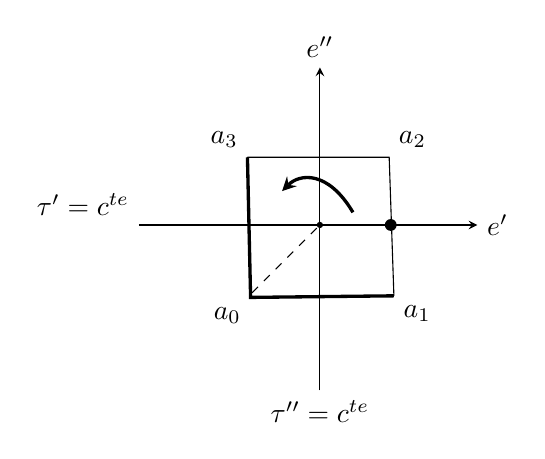
\begin{tikzpicture}[x=1cm,y=1cm,>=stealth]
\draw[->] (-2.3,0)--(2,0) node[right] {$e'$};
\draw[->] (0,-2.1)--(0,2) node[above] {$e''$};
\draw (-.92,.86)--(.88,.86)--(.94,-.9);
\draw[very thick] (-.92,.86)--(-.88,-.92)--(.94,-.9);
\draw[dashed] (-.86,-.86)--(0,0); \fill (0,0) circle (.04); \fill (.9,0) circle (.075);
\draw[->,very thick] (.42,.16) .. controls (.1,.7) and (-.26,.65) .. (-.48,.43);
\node[above left] at (-.92,.86) {$a_3$}; \node[above right] at (.88,.86) {$a_2$};
\node[below left] at (-.88,-.92) {$a_0$}; \node[below right] at (.94,-.9) {$a_1$};
\node[above left] at (-2.3,0) {$\tau'=c^{te}$}; \node[below] at (0,-2.1) {$\tau''=c^{te}$};
\end{tikzpicture}}
\[
\left\{\begin{array}{ll}
\tau'e'=e' & \tau''e'=-e'\\
\tau'e''=-e'' & \tau''e''=e''\\[.7em]
\sigma e'=e'' & \sigma e''=-e'
\end{array}\right.
\]
\[
\begin{gathered}
\tau'\tau''=\tau''\tau'=\sigma^2\deleted{\unsure{\infty}}=\omega_0\\
\sigma^4=\omega_0^2=1\\
\deleted{\unsure{\sigma\tau''=\tau''\sigma}}\\
\deleted{\unsure{\tau'\varepsilon_0}}
\end{gathered}
\]
\margin{$\left\{\begin{array}{l}\omega_0e'=-e'\\\omega_0e''=-e''\end{array}\right.$}
\[
\begin{array}{ll}
\sigma\tau'=\tau'_\infty=r_0 &: \quad e'\longmapsto e''\\
\Vert &\quad e''\mathrel{\mapstochar\relbar\relbar\mapstochar}e'\\
\tau'\sigma^{-1} &\\
\Vert &\\
\sigma^{-1}\tau''=\tau''\sigma&\\
(\tau'=\sigma^2\tau''&
\end{array}
\]
\[
\begin{array}{l}
\tau''\longmapsto\tau_\infty=r_\infty\\
\sigma\longmapsto\sigma=\sigma_\infty\\
\varepsilon'\longmapsto\varepsilon_0\\
\varepsilon''=\sigma(\varepsilon')\mathrel{\mapstochar\relbar\relbar\mapstochar}\varepsilon_1
\end{array}
\qquad
\begin{array}{l}
\varepsilon'(e')=e'\\
\varepsilon'e''=e''-e'
\end{array}
\]
\margin{$\varepsilon'$ était $\rho'$ avant}
\[
\begin{array}{l}
\varepsilon_0=\sigma\rho\quad\varepsilon_1=\rho\sigma\\
\varepsilon_1\varepsilon_0=-\rho^2=\rho^{-1}\\
\deleted{-\varepsilon_1\varepsilon_0=\omega_0\varepsilon_1\varepsilon_0=}
\end{array}
\qquad
\left\{\begin{array}{l}
\sigma(\varepsilon')=\varepsilon''\\
\tau'(\varepsilon')=\tau''(\varepsilon')=\varepsilon^{\prime-1}\\
\tau'(\varepsilon'')=\tau''(\varepsilon'')=\varepsilon^{\prime\prime-1}
\end{array}\right.
\]
\deleted{$\unsure{\varepsilon_0}\quad\varepsilon_1\varepsilon_0=\unsure{\rho_0}$}
\[
\left\{\begin{array}{l}
\rho=(\varepsilon_1\varepsilon_0)^{-1}=\varepsilon_0^{-1}\varepsilon_1^{-1}\\
\sigma_\infty=\varepsilon_0\rho^{-1}=\varepsilon_0\varepsilon_1\varepsilon_0=\rho^{-1}\varepsilon_1=\varepsilon_1\varepsilon_0\varepsilon_1\\
\deleted{\unsure{\tau_0}}\quad r_0(\varepsilon_0)=\varepsilon_1^{-1}\\
r_0(\varepsilon_1)=\varepsilon_0^{-1}
\end{array}\right.
\]
\margin{$\deleted{\unsure{\varepsilon_0\varepsilon_1}}$}
\[
\left[\begin{array}{l}
r_0(\rho)=\varepsilon_1\varepsilon_0=\rho^{-1}\\
r_0(\sigma)=\varepsilon_1^{-1}\varepsilon_0^{-1}\varepsilon_1^{-1}=\varepsilon_0^{-1}\varepsilon_1^{-1}\varepsilon_0^{-1}
\end{array}\right.
\]
\[
\varepsilon_0,\varepsilon_1,\unsure{\tau_0|r_0}
\]
\margin{i.e. $\begin{gathered}
\varepsilon_1\varepsilon_0\varepsilon_1=\varepsilon_0\varepsilon_1\varepsilon_0\\
\rho\sigma\sigma\rho\rho\sigma=\sigma\rho\rho\sigma\sigma\rho\\
\deleted{\unsure{\varepsilon_1\underbrace{\varepsilon_0\varepsilon_1\varepsilon_0\varepsilon_1^{-1}}_{\longleftarrow}\varepsilon_0^{-1}}}\\
\rho\sigma^2\rho^2\sigma=\sigma\rho^2\sigma^2\rho\\
-\underbrace{\rho^3\sigma}_{\sigma}=-\underbrace{\sigma\rho^3}_{\sigma}
\end{gathered}$}

\margin{160}


\scanpage{161}
UNIVERSITE\\
DES SCIENCES ET TECHNIQUES\\
DU LANGUEDOC\\
------------

MONTPELLIER, le 16 septembre 1980

Service de la Scolarité\\
MA/IE\\
\uline{Diffusion} : liste A\\
N° 4583

\uline{AVIS DE SOUTENANCE D'UNE THESE DE DOCTORAT DE 3ème CYCLE} :

\uline{AGRONOMIE Option ZOOTECHNIE}

\uline{Nom et prénom du candidat} : JIMENEZ Nelys épouse PEREZ

\uline{Titre de la thèse} : Effets de la gestation et du mode de conduite (traite ou allaitement) sur la durée de l'anoestrus post-partum chez la vache française Frisonne Pie noire (FFPN).

\uline{Date, heure et lieu de soutenance prévus} : 26 septembre 1980 à 9 H 30, laboratoire de Zootechnie, ENSAM, Montpellier

\uline{Nom du Directeur de la thèse} : MM. DAUZIER et MAULEON

\uline{Désignation du laboratoire où la thèse est préparée} : laboratoire de Physiologie de la Reproduction - INRA - Nouzilly

\uline{Analyse de l'ouvrage} : Sur 80 vaches Frisonnes Pie noire (FFPN) une caractérisation hormonale pré et post-partum a été faite en comparant deux modes de conduite : traite ou allaitement.

L'importance du rôle de l'utérus dans la reprise de l'activité ovarienne a été \deleted{\unsure{le}} mise en évidence grâce à la mesure dans le sang du métabolite de la $\mathrm{PGF}_2\alpha$ (PGFM).

Le rôle déterminant du système nerveux dans cette reprise a été confirmé par l'étude objective des variations plasmatiques de LH.

Variations de concentration plasmatique de LH, niveau de prostaglandine F2$\alpha$ et prolactinémie expliquent 40 \% de la variabilité de l'intervalle vêlage-1ère ovulation. Des corrélations entre paramètres pre-partum et post-partum suggèrent qu'une partie des variations est issue des situations physiologiques pendant la gestation.

Les résultats montrent clairement l'effet \unsure{négatif|néggatif} sur la reprise de l'activité ovarienne de l'allaitement en comparaison avec la traite.

\uline{Durée approximative des recherches ayant abouti à la thèse} : 3 ans.

\uline{Composition du jury proposé} : MM. : DAUZIER\\
LEGRAND\\
MAULEON\\
VEZINHET

P/le Secrétaire Général\\
L'Attachée d'Administration Universitaire,

\figure{
\begin{tikzpicture}[x=1cm,y=1cm]
\draw (0,0) .. controls (-.08,.25) and (.24,.5) .. (.19,.71) .. controls (.12,.83) and (.02,.31) .. (.07,.17) .. controls (.18,.01) and (.15,.37) .. (.01,.36) .. controls (-.08,.3) and (.03,.01) .. (.04,-.04);
\end{tikzpicture}}
\uline{\unsure{Gentil}}\\
\uline{GENTIL}

MR LE PROFESSEUR GROTHENDIECK ALEX.\\
MATHEMATIQUES\qquad5

\margin{161}


\scanpage{162}
\margin{162}
\figure{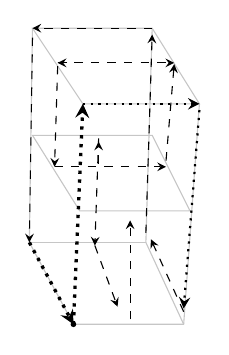
\begin{tikzpicture}[x=.8cm,y=.8cm,>=stealth]
\draw[gray!45] (0,4.7)--(1.9,4.7)--(2.65,3.5)--(.8,3.5)--cycle;
\draw[gray!45] (0,4.7)--(-.05,1.3)--(.65,0)--(2.4,0)--(2.65,3.5);
\draw[gray!45] (1.9,4.7)--(1.8,1.3)--(2.4,0);
\draw[gray!45] (0,3)--(1.9,3)--(2.5,1.8)--(.75,1.8)--cycle;
\draw[gray!45] (-.05,1.3)--(1.8,1.3);
\draw[->,dashed] (1.9,4.7)--(0,4.7); \draw[->,dashed] (0,4.55)--(-.05,1.3);
\draw[->,dashed] (1.8,1.45)--(1.9,4.6);
\draw[->,dashed] (.4,4.15)--(2.25,4.15); \draw[->,dashed] (.55,4.15)--(.4,4.15);
\draw[->,dashed] (.4,4.1)--(.35,2.5); \draw[->,dashed] (.35,2.5)--(2.12,2.5);
\draw[->,dashed] (2.12,2.6)--(2.25,4.13);
\draw[->,dotted,very thick] (-.05,1.3)--(.65,0);
\draw[->,dotted,very thick] (.65,0)--(.8,3.5); \draw[->,dotted,thick] (.8,3.5)--(2.65,3.5);
\draw[->,dotted,thick] (2.65,3.4)--(2.4,.25);
\draw[->,dashed] (1.05,2.95)--(.99,1.25); \draw[->,dashed] (1.05,2.55)--(1.05,2.9);
\draw[->,dashed] (.99,1.25)--(1.35,.28); \draw[->,dashed] (1.55,.08)--(1.55,1.65);
\draw[->,dashed] (2.4,.2)--(1.88,1.35);
\fill (.65,0) circle (.045);
\end{tikzpicture}}

\figure{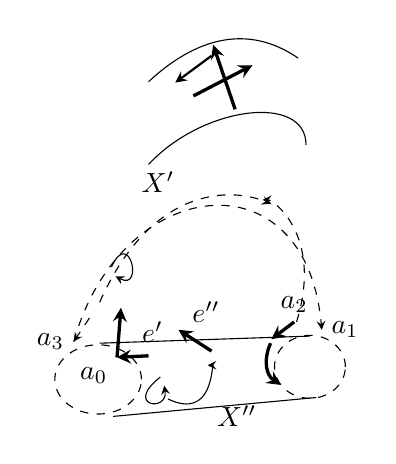
\begin{tikzpicture}[x=1cm,y=1cm,>=stealth]
\draw (-.7,3.45) .. controls (0,4.1) and (.65,4.13) .. (1.2,3.75);
\draw (-.7,2.4) .. controls (0,3.15) and (1.3,3.3) .. (1.3,2.65);
\draw[->,very thick] (.4,3.1)--(.12,3.92);
\draw[->,thick] (.1,3.78)--(-.36,3.44); \draw[->,very thick] (-.13,3.27)--(.62,3.66);
\draw[dashed,->] (-1.65,.15) .. controls (-1.05,2.28) and (1.3,2.55) .. (1.5,.3);
\draw[dashed,->] (-1.32,.65) .. controls (-.65,2.16) and (.38,2.1) .. (.85,1.9);
\draw[dashed,->] (1.18,.4) .. controls (1.52,1.5) and (.88,1.95) .. (.75,1.95);
\draw[dashed,->] (-1.45,.45)--(-1.65,.15);
\draw[dashed] (-1.34,-.33) ellipse (.55 and .44); \draw[dashed] (1.35,-.17) ellipse (.45 and .4);
\draw (-1.32,.13)--(1.35,.22); \draw (-1.15,-.8)--(1.43,-.56);
\draw[->,very thick] (-.7,-.03)--(-1.1,-.05); \draw[->,very thick] (-1.1,-.05)--(-1.05,.58);
\draw[->,very thick] (.1,.03)--(-.32,.3); \draw[->,very thick] (1.15,.4)--(.86,.18);
\draw[->,very thick] (.85,.13) .. controls (.75,-.1) and (.8,-.28) .. (.98,-.4);
\draw[->] (-.45,-.58) .. controls (.12,-.85) and (.1,-.15) .. (.05,-.15);
\draw[->] (-.55,-.3) .. controls (-1.02,-.67) and (-.45,-.75) .. (-.5,-.41);
\draw[->] (-1.17,1.1) .. controls (-.94,1.6) and (-.76,.79) .. (-1.12,.98);
\node at (-.58,2.18) {$X'$}; \node at (.42,-.8) {$X''$};
\node[left] at (-1.65,.15) {$a_3$}; \node[below left] at (-1.1,-.05) {$a_0$};
\node[above] at (1.15,.4) {$a_2$}; \node[right] at (1.5,.3) {$a_1$};
\node[above] at (-.65,.01) {$e'$}; \node[above] at (.03,.27) {$e''$};
\end{tikzpicture}}

\[
X'_{\unsure{\varepsilon|s}}\qquad X''_{\unsure{\varepsilon|s}}
\]
\diagram{\[
\left.\begin{array}{ccc}
\varepsilon_0(\unsure{X'|X}) &\xrightarrow{\sim}& \varepsilon_1(X'')\\
\varepsilon_1(X') &\xleftarrow{\sim}& \varepsilon_0(X'')
\end{array}\right\}\quad\Downarrow
\]}
\rule{5.8cm}{.4pt}
\diagram{\begin{tikzcd}[column sep=small,row sep=small]
\omega(X')\arrow[rr,no head,"\simeq"]\arrow[dr] && \omega(X'')\arrow[dl]\\
&\overset{\ominus}{\omega(X'\wedge X'')}&\begin{gathered}\text{anticommu-}\\\text{tatif}\end{gathered}
\end{tikzcd}}

$\tau',\tau'',\sigma$ ne dépendent que du ``\unsure{carré|cône} d'orientations''

$e',\ e''$ fixent les 1-orientations et aussi une \unsure{2-orientation|2-orientations} sur \uuline{chaque} \uline{morceau} $X',X''$, d'où $\rho',\rho''$
\[
\begin{array}{ll}
\tau'e'=e' & \tau''e'=-e'\\
\tau'e''=-e'' & \tau''e''=+e''
\end{array}
\]
\figure{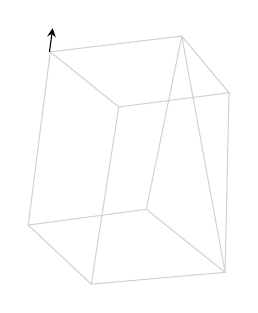
\begin{tikzpicture}[x=1cm,y=1cm,>=stealth]
\draw[gray!35] (0,0)--(1.5,.2)--(2.5,-.6)--(.8,-.75)--cycle;
\draw[gray!35] (0,0)--(.28,2.2)--(1.95,2.4)--(2.5,-.6);
\draw[gray!35] (1.5,.2)--(1.95,2.4); \draw[gray!35] (.8,-.75)--(1.15,1.5)--(2.55,1.68)--(1.95,2.4);
\draw[gray!35] (.28,2.2)--(1.15,1.5); \draw[gray!35] (2.55,1.68)--(2.5,-.6);
\draw[->] (.27,2.2)--(.31,2.5);
\end{tikzpicture}}

d'où $\rho',\rho''$
\[
\left\{\begin{array}{l}
\tau'(\rho')=\tau''(\rho')=\rho^{\prime-1}\\
\tau^{\unsure{''|'}}(\rho'')=\tau''(\rho'')=\rho^{\prime\prime-1}\\
\sigma(\rho')=\rho'',\quad\sigma\rho''=\rho'
\end{array}\right.
\]
\margin{$\begin{aligned}\rho'(e')&=e'\\\rho'(e'')&=-e'+e''\end{aligned}$}

\margin{M. \uline{Grothendieck}}


\scanpage{163}
UNIVERSITE DES SCIENCES ET TECHNIQUES\\
DU LANGUEDOC\\
---

INSTITUT DE MATHEMATIQUES\\
Place Eugène Bataillon\\
34060 MONTPELLIER CEDEX\\
---

Montpellier, le 24 septembre 1980

\uline{DEUG A - 1ère Année - Série III}

Convocation de jury :

LUNDI 29 septembre 1980 - 14 h 30 - Salle 2TC1P

M. VALADIER

\margin{163}


\scanpage{164}

\[
\tau',\ \uline{\tau''},\ \uline{\sigma},\ \uline{\rho'},\ \rho''
\qquad \deleted{\unsure{\sigma|\tau}}
\]
\[
\left\{\begin{aligned}
&\tau'^2=\tau''^2=\sigma^4=1\qquad \sigma^2=\tau'\tau'',\quad
 \deleted{\sigma(\rho')=\rho}\\
&\tau'(\rho')=\tau''(\rho')=\rho'^{-1},\qquad
 \unsure{\tau'|\tau''}(\rho'')=\tau''(\rho'')=\rho''^{-1}\\
&\sigma(\rho')=\rho''\qquad(\Rightarrow\sigma(\rho'')=\rho')\\
&(\sigma\rho')^3\unsure{\sim|\simeq}1\quad\text{dans }\mathcal T^+_{1,1}
\end{aligned}\right.
\]
\hfill (mais \inserted{non} dans un groupe spécial)

\diagram{\[
\begin{array}{rcl|l}
\rho'&\longmapsto&\varepsilon_0&\\
\rho''&\mathrel{\mapstochar\! -\! -}&\varepsilon_1&\\[3pt]
\tau''&\longmapsto&\tau_\infty=\tau=r_\infty&\\[3pt]
\tau'&\longmapsto&\omega_0\tau_\infty=-\tau&\\[3pt]
\sigma&\mathrel{\mapstochar\! -\! -}&\sigma_\infty=\sigma&
\end{array}
\]}

\[
\sigma^{-1}\rho'=\sigma^3\rho'\longmapsto
 \sigma^3\varepsilon_0=\sigma^3(\sigma\rho)=\rho
\]
\[
\tau''\sigma\longmapsto\tau'_\infty=r_0
\]
\[
\tau''\rho'=\underbrace{(\tau''\sigma)}_{\mapsto r_0}
 \underbrace{(\sigma^{-1}\rho')}_{\mapsto\rho}
 \mathrel{\mapstochar\! -\! -}r_1
\]

\diagram{\[
\begin{array}{|rcl|rcl|}\hline
\tau''&\longmapsto&r_\infty&\rho'&\mathrel{\mapstochar\! -\! -}&\varepsilon_0\\
\tau''\sigma&\longmapsto&r_0&\sigma&\longmapsto&\sigma\\
\tau''\rho'&\longmapsto&r_1&\sigma^{-1}\rho'&\mathrel{\mapstochar\! -\! -}&\rho\\\hline
\end{array}
\]}
\[
\unsure{\mathfrak X|\mathcal X}=(X,X',X'')
\]

\figure{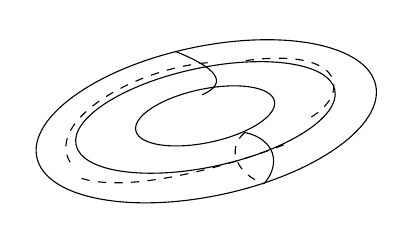
\begin{tikzpicture}[x=1cm,y=1cm,rotate=12]
\draw (0,0) ellipse (2.2 and .95);
\draw (0,.05) ellipse (1.68 and .63);
\draw (0,.07) ellipse (.9 and .34);
\draw[dashed] (-1.8,-.15) .. controls (-2,.45) and (-.7,.85) .. (.2,.72);
\draw[dashed] (.65,.65) .. controls (1.95,.55) and (1.85,-.05) .. (1.3,-.23);
\draw[dashed] (-1.7,-.38) .. controls (-1.1,-.72) and (.35,-.6) .. (1,-.48);
\draw (-.2,.95) .. controls (.25,.65) and (.4,.42) .. (.02,.34);
\draw (.45,-.24) .. controls (.8,-.4) and (.83,-.72) .. (.55,-.93);
\draw[dashed] (.45,-.24) .. controls (.16,-.4) and (.25,-.74) .. (.55,-.93);
\end{tikzpicture}}

\figure{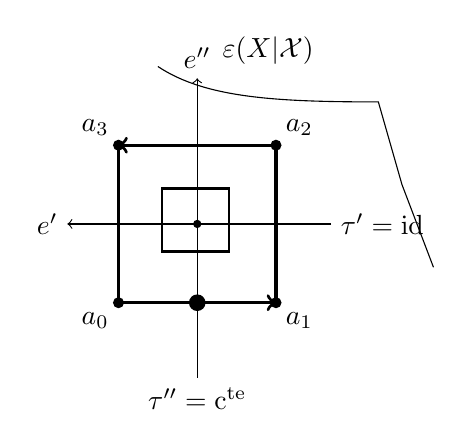
\begin{tikzpicture}[x=1cm,y=1cm]
\draw[very thick] (0,0) rectangle (2,2);
\draw[very thick,->] (0,0)--(2,0);
\draw[very thick,->] (2,2)--(0,2);
\draw[thick] (.55,.65) rectangle (1.4,1.45);
\draw[->] (2.7,1)--(-.65,1) node[left] {$e'$};
\draw[->] (1,-.95)--(1,2.85) node[above] {$e''$};
\fill (0,0) circle (2pt) node[below left] {$a_0$};
\fill (2,0) circle (2pt) node[below right] {$a_1$};
\fill (2,2) circle (2pt) node[above right] {$a_2$};
\fill (0,2) circle (2pt) node[above left] {$a_3$};
\fill (1,0) circle (3pt);\fill (1,1) circle (1.5pt);
\node[right] at (2.7,1) {$\tau'=\mathrm{id}$};
\node[below] at (1,-.95) {$\tau''=\mathrm{c}^{\mathrm{te}}$};
\node at (1.9,3.2) {$\varepsilon(\unsure{\mathfrak X|\mathcal X})$};
\draw (.5,3) .. controls (1.1,2.6) and (2,2.55) .. (3.3,2.55)
 --(3.6,1.5)--(4,.45);
\end{tikzpicture}}

$\{X',X''\}={}$ ens des codiagonales du carré

$\varepsilon_0(X')\simeq{}$ ens des deux côtés opposés du carré qui correspondent à \unsure{le|la} $X''$

$\varepsilon_1(X')\simeq{}$ ens des deux côtés opposés du carré qui correspondent à $X'$

\margin{$\varepsilon(\unsure{\mathfrak X|\mathcal X})\ \deleted{\unsure{\varepsilon_0(X')|\varepsilon_1(X')}}$}
\margin{\deleted{\unsure{faut|font}}}

\[
\begin{aligned}
\varepsilon_0(X')\times\varepsilon_1(X')&\simeq
 \text{ens des \deleted{\unsure{deux côtés}} \inserted{sommets} du carré}\\
&\simeq\varepsilon_1(X'')\times\varepsilon_0(X'')\\
&\simeq\varepsilon_0(X')\times\varepsilon_0(X'').\\
&\deleted{\simeq\unsure{\varepsilon_0|\varepsilon_1}(X'')\times\varepsilon}
 \simeq\varepsilon_1(X')\times\varepsilon_1(X'')
\end{aligned}
\]
\margin{164}


\scanpage{165}

\begin{flushleft}
U N I V E R S I T E\\
DES SCIENCES ET TECHNIQUES\\
DU LANGUEDOC\\
------------\\
Service de la Scolarité\\
MA/IE\\
\uline{Diffusion} : liste A\\
n°4584
\end{flushleft}
\begin{flushright}MONTPELLIER, le 16 septembre 1980\end{flushright}

\begin{center}
\uline{AVIS DE SOUTENANCE D'UNE THESE DE DOCTORAT DE 3ème CYCLE} :

\uline{AGRONOMIE Option ZOOTECHNIE}
\end{center}

\uline{Nom et prénom du candidat} : PEREZ MURUA Oscar

\uline{Titre de la thèse} : Influence du mode de conduite sur le comportement maternel et quelques paramètres zootechniques chez la vache Française Frisonne Pie Noire (FFPN) en lactation.

\uline{Date, heure et lieu de soutenance prévus} : 26 septembre 1980 à 14 H 30 au laboratoire de Zootechnie - ENSAM, Montpellier

\uline{Nom du Directeur de la thèse} : Monsieur le Professeur DAUZIER

\uline{Désignation du laboratoire où la thèse est préparée} : laboratoire de Physiologie de la Reproduction, INRA Nouzilly

\uline{Analyse de l'ouvrage} : Nous avons étudié le comportement maternel des vaches soumises à 3 modes de conduite : allaitement libre de 3 veaux par vache après une période d'adoption, allaitement surveillé de 3 veaux par vache deux fois par jour et traite deux fois par jour.

Nous avons trouvé une influence sur le comportement maternel, la production laitière et le taux de prolactine dans le sang lors de la stimulation mammaire selon le mode de conduite des vaches. Egalement, la croissance des veaux a été affectée par la qualité de l'adoption.

\uline{Durée approximative des recherches ayant abouti à la thèse} : 3 ans.

\uline{Composition du jury proposé} : MM. : \begin{tabular}[t]{l}
DAUZIER\\
SIGNORET\\
LEGRAND\\
PRUD'HON
\end{tabular}

\begin{flushright}
P/le Secrétaire Général\\
L'Attachée d'Administration Universitaire,

\figure{
\begin{tikzpicture}[x=1cm,y=1cm]
\draw (0,0) .. controls (-.08,.25) and (.24,.5) .. (.19,.71) .. controls (.12,.83) and (.02,.31) .. (.07,.17) .. controls (.18,.01) and (.15,.37) .. (.01,.36) .. controls (-.08,.3) and (.03,.01) .. (.04,-.04);
\end{tikzpicture}}
\uline{\unsure{Gentil}}\\
\uline{A. GENTIL}
\end{flushright}

\margin{165}


\scanpage{166}

\[
\left\{\begin{aligned}
&\sigma_1^2=\sigma_2^2=(\sigma_1\sigma_2)^2=1\\
&\rho_1,\rho_{\unsure{2|\infty}}
\end{aligned}\right.
\]
\[
\sigma_i\rho_j=\rho_{\unsure{j|2}}^{-1}
\]
\[
\begin{aligned}
\widetilde\tau\widetilde\rho&=\widetilde\rho^{-1}\\
\widetilde\tau\widetilde\sigma&=\widetilde\sigma^{-1}
\end{aligned}
\qquad\widetilde\rho^3\,-
\]

\figure{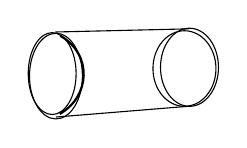
\begin{tikzpicture}[x=.8cm,y=.8cm]
\draw (0,0) ellipse (.38 and .65);
\draw (.06,-.04) ellipse (.42 and .68);
\draw (2.1,.08) ellipse (.5 and .6);
\draw (2.18,.1) ellipse (.46 and .62);
\draw (.05,.66)--(2.17,.71);\draw (.06,-.69)--(2.15,-.52);
\draw[thick] (.13,.6) .. controls (.65,.3) and (.6,-.37) .. (.12,-.64);
\end{tikzpicture}}

\figure{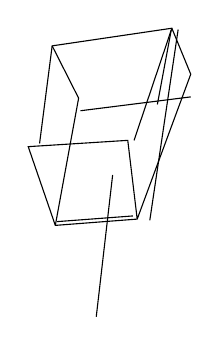
\begin{tikzpicture}[x=.8cm,y=.8cm]
\draw (-.1,.1)--(.1,1.65)--(2,1.93)--(2.3,1.2)--(1.45,-1.1)--(.15,-1.2)--(-.28,.05)--(1.3,.15)--(1.45,-1.1);
\draw (.1,1.65)--(.52,.82)--(.15,-1.2);
\draw (.55,.62)--(2.3,.84);\draw (2,1.93)--(1.4,.15);
\draw (2.1,1.91)--(1.65,-1.12);\draw (1.99,1.9)--(1.77,.72);
\draw (.18,-1.14)--(1.38,-1.05);\draw (1.06,-.4)--(.8,-2.65);
\end{tikzpicture}}

\figure{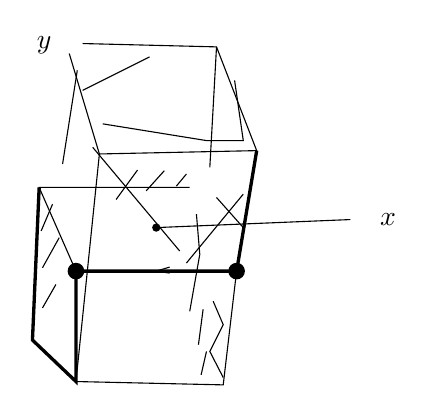
\begin{tikzpicture}[x=.85cm,y=.85cm]
\draw (0,2.9)--(.45,1.4)--(2.8,1.45)--(2.2,3)--(.2,3.05);
\draw (.12,2.65)--(-.1,1.25);
\draw (.45,1.4)--(.1,-2)--(-.55,-1.38)--(-.45,.9)--(1.8,.9);
\draw[very thick] (-.45,.9)--(-.55,-1.38)--(.1,-2)--(.1,-.35)--(2.5,-.35)--(2.8,1.45);
\draw (.1,-2)--(2.3,-2.05)--(2.5,-.35);
\draw (-.45,.9)--(.1,-.35);\draw (2.2,3)--(2.1,1.2);
\draw (.5,1.85)--(2.05,1.6)--(2.6,1.6)--(2.47,2.5);
\draw (.2,2.35)--(1.2,2.85);\draw (.35,1.5)--(1.65,-.05);
\draw (1.3,.3)--(4.2,.42);\fill (1.3,.3) circle (1.5pt);
\fill (.1,-.35) circle (3pt);\fill (2.5,-.35) circle (3pt);
\draw (1.5,-.38)--(1.3,-.35)--(1.5,-.29);
\draw (1.95,-.1)--(1.9,.5);\draw (1.95,-.1)--(1.8,-.95);
\draw (2.6,.8)--(1.75,-.23);\draw (2.2,.75)--(2.6,.3);
\draw (2.15,-.8)--(2.3,-1.15)--(2.1,-1.55)--(2.3,-1.94);
\draw (2,-.92)--(1.93,-1.45);\draw (2.05,-1.55)--(1.97,-1.9);
\draw (-.42,.25)--(-.25,.65);\draw (-.4,-.3)--(-.15,.15);\draw (-.4,-.9)--(-.2,-.55);
\draw (.7,.72)--(1.02,1.16);\draw (1.15,.85)--(1.42,1.15);\draw (1.6,.92)--(1.75,1.1);
\node[left] at (-.12,3.02) {$y$};\node[right] at (4.5,.42) {$x$};
\end{tikzpicture}}

\figure{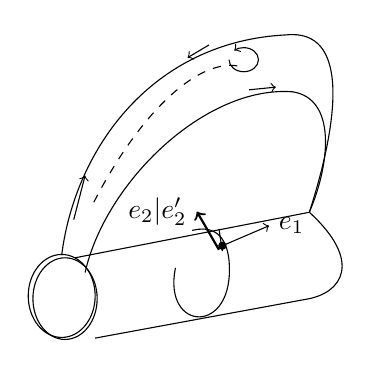
\begin{tikzpicture}[x=.85cm,y=.85cm]
\draw (0,0) ellipse (.5 and .62);
\draw (.05,-.04) ellipse (.48 and .61);
\draw (.2,.57)--(3.7,1.25) .. controls (4.5,.52) and (4.2,.04) .. (3.65,-.05)--(.5,-.63);
\draw (0,.61) .. controls (.2,2.2) and (1.35,3.8) .. (3.35,3.9)
 .. controls (4.3,4) and (4.15,2.65) .. (3.7,1.25);
\draw (.35,.35) .. controls (.65,1.7) and (2.15,3.15) .. (3.45,3.05)
 .. controls (4.1,2.95) and (4.02,2) .. (3.7,1.25);
\draw[dashed] (.48,1.4) .. controls (1.2,2.8) and (2.1,3.6) .. (2.7,3.42);
\draw[->] (.18,1.14)--(.35,1.8);\draw[->] (2.2,3.75)--(1.88,3.56);
\draw[->] (2.8,3.08)--(3.2,3.12);
\draw[->] (2.5,3.53) arc[start angle=180,end angle=490,x radius=.22,y radius=.18];
\draw (1.7,.42) .. controls (1.5,-.55) and (2.6,-.6) .. (2.5,.53)
 .. controls (2.45,1.02) and (2.15,1.03) .. (1.95,.98);
\draw[->] (2.4,.75)--(3.1,1.05) node[right] {$e_1$};
\draw[->,thick] (2.35,.69)--(2.02,1.26) node[left] {$\unsure{e_2|e'_2}$};
\draw (2.4,.67)--(2.35,1);\fill (2.4,.75) circle (1.5pt);
\end{tikzpicture}}

\[
x\mathrel{\mapstochar\! -\! -}-x\qquad
 y\longmapsto y
\]
\[
(x,y,z)\longmapsto\unsure{ix|iX},
\]
\[
(z,t)\longrightarrow(iz,-t)
\]

\figure{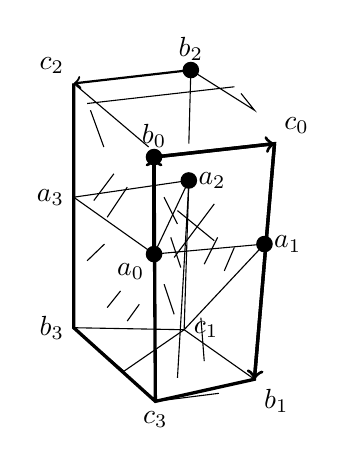
\begin{tikzpicture}[x=.85cm,y=.85cm]
\coordinate (c2) at (0,3.8);\coordinate (b2) at (1.75,4);
\coordinate (a3) at (0,2.1);\coordinate (b3) at (0,.15);
\coordinate (b0) at (1.2,2.7);\coordinate (c0) at (3,2.9);
\coordinate (a0) at (1.2,1.25);\coordinate (a1) at (2.85,1.4);
\coordinate (a2) at (1.72,2.35);\coordinate (c1) at (1.65,.12);
\coordinate (b1) at (2.7,-.62);\coordinate (c3) at (1.22,-.95);
\draw[very thick] (c2)--(b3)--(c3)--(b1)--(c0)--(b0)--(c3);
\draw[very thick,->] (b0)--(c0);\draw[very thick,->] (c0)--(b1);
\draw[very thick,->] (a0)--(b0);\draw[thick,->] (b2)--(c2);
\draw (b2)--(1.72,2.9);\draw (c2)--(1.12,2.85);\draw (b2)--(2.7,3.4)--(2.5,3.65);
\draw (a3)--(a2)--(a0)--(a1)--(c1)--(b3);\draw (a2)--(c1);
\draw (c1)--(b1);\draw (c3)--(2.17,-.83);\draw (a3)--(a0);
\draw (b3)--(.75,-.5)--(c1);\draw (.2,3.5)--(2.4,3.75);
\draw (.25,3.4)--(.45,2.85);\draw (.3,2.05)--(.6,2.45);\draw (.5,1.8)--(.8,2.25);
\draw (.2,1.15)--(.46,1.4);\draw (.5,.45)--(.7,.7);\draw (.8,.25)--(.98,.5);
\draw (1.35,2.1)--(1.55,1.7);\draw (1.45,1.5)--(1.6,1.05);
\draw (1.35,.8)--(1.5,.35);\draw (1.95,1.1)--(2.15,1.5);\draw (2.25,1)--(2.4,1.35);
\draw (1.9,.3)--(1.95,-.35);\draw (1.72,2.3)--(1.55,-.6);
\draw (1.55,1.9)--(2.1,1.45);\draw (1.5,1.2)--(2.1,2);
\foreach \p in {a0,a1,a2,b0,b2} {\fill (\p) circle (3pt);}
\node[above left] at (c2) {$c_2$};\node[above] at (b2) {$b_2$};
\node[left] at (a3) {$a_3$};\node[left] at (b3) {$b_3$};
\node[above] at (b0) {$b_0$};\node[above right] at (c0) {$c_0$};
\node[below left] at (a0) {$a_0$};\node[right] at (a1) {$a_1$};
\node[right] at (a2) {$a_2$};\node[right] at (c1) {$c_1$};
\node[below right] at (b1) {$b_1$};\node[below] at (c3) {$c_3$};
\end{tikzpicture}}

\[
\sigma\varphi
\qquad \deleted{\unsure{\mathbb Z_2|\mathbb Z/2}}\unsure{D_\sigma|D\sigma}
\]
\[
\boxed{\sigma^2=\sigma_1\sigma_2=\boxed{\sigma_2\sigma_1}}
\]
\[
\sigma_1^2=\sigma_2^2\quad(=\sigma^4)=1
\]
\[
\begin{aligned}
\sigma_1(\sigma)&=\sigma^{-1}\\
\sigma_2(\sigma)&=\sigma^{-1}
\end{aligned}\qquad ?
\]
\[
\deleted{(\sigma_1,\sigma_2)}\qquad\deleted{(\sigma_1\sigma_2)^2}
\]
\[
\begin{aligned}
\sigma(z,t)&=\unsure{(iz|(z},-t)\\
\sigma_1(z,t)&=(\overline z,t)\\
\sigma_2(z,\unsure{t|h})&=(-\overline z,t)
\end{aligned}
\]
\[
\sigma_2=\sigma_1\sigma^2=\sigma^2\sigma_1
\]
\[
\begin{pmatrix}1&1\\0&1\end{pmatrix}\qquad
\begin{pmatrix}1&-1\\0&1\end{pmatrix}
\]
\[
(z,t)\mathrel{\mapstochar\! -\! -}(\overline z,t)
 \mathrel{\mapstochar\! -\! -}(i\overline z,-t)
 \longmapsto(-iz,-t)
\]
\margin{166}


\scanpage{167}

\begin{flushleft}
UNIVERSITE DES SCIENCES\\
ET TECHNIQUES DU LANGUEDOC\\
MATHEMATIQUES
\end{flushleft}
\begin{flushright}22.10.80\end{flushright}

\begin{center}
SEMINAIRE D'ANALYSE CONVEXE

Jeudi 30 Octobre 1980 à 10 h 30, Salle 431

J. CEA, Professeur, Université de Nice
\end{center}

\uline{\unsure{Méthode'|Méthode} de décomposition utilisant des opérateurs intégraux.}

Applications aux problèmes avec coin, aux problèmes \unsure{extérieurs|extérieure}, au bilaplacien.

A 14 h 15, le même jour, Salle 431

\begin{center}R. GONZALEZ DE PAZ\end{center}

soutiendra sa thèse de 3e cycle,

\begin{center}
Sur un problème d'optimisation de domaine.

\rule{3cm}{.4pt}
\end{center}

\margin{167}

